\documentclass[12pt, oneside]{article}   	% use "amsart" instead of "article" for AMSLaTeX format
%\documentclass[12pt, oneside, draft]{article}   	% use "amsart" instead of "article" for AMSLaTeX format

%%%%%%%%%%%%%%%%%%%%%%%%%%%%%%%%%%%%%%%%%%%%%%%%%
%
% The TexLive distribution is stored in /usr/local/texlive/2020
%
% The definitions of the packages are in /usr/local/texlive/2020/texmf-dist/tex/latex
%
%%%%%%%%%%%%%%%%%%%%%%%%%%%%%%%%%%%%%%%%%%%%%%%%%

\usepackage{xparse}					% Allows for the creation of \NewDocumentCommand shortcuts

\usepackage{geometry}				% See geometry.pdf to learn the layout options. There are lots.
\geometry{letterpaper}				% ... or a4paper or a5paper or ... 
\usepackage[parfill]{parskip}		% Activate to begin paragraphs with an empty line rather than indent
\usepackage{float}					% Float package to exert more control over graphic placement
	
% Math packages
\usepackage{amssymb}				% Mathematical symbols
\usepackage{amsmath}				% Added for typesetting mathematical formulae
\usepackage{amsthm}					% Added for typesetting mathematical theorems
\usepackage{mathalpha}				% Added for some special characters like Q, Z and N

% Table packages in addition to built in tabular
\usepackage{booktabs}				% Adds extra commands to tabular like \toprule
\usepackage{afterpage}				% For pagination support

% Hyperlinks
\usepackage{hyperref}				% For creating internal and HTTP links

% Numbering and references
\numberwithin{equation}{section}          % Number equations within sections
\usepackage[numbers]{natbib}              % For bibliography management

% For Tikz graphics
\usepackage{tikz}					% Package for pgf and TikZ
\usetikzlibrary{shapes,arrows,chains}
\tikzstyle{startstop} = [very thick, rectangle, rounded corners, minimum width=2.5cm, minimum height=0.8cm, text centered, draw=black, text width=2.5cm]
\tikzstyle{action} = [rectangle, rounded corners, minimum width=3cm, minimum height=0.8cm, text centered, draw=black, text width=2.5cm]
\tikzstyle{decision} = [diamond, minimum width=3cm, minimum height=3cm, text centered, draw=black, text width=2cm]
\tikzstyle{arrow} = [thick,->,>=stealth]

% For theorems and definitions - each creates it's own counter which incrementa each use
\theoremstyle{definition}
\newtheorem{proposition}{Proposition}[section]
\newtheorem{define}{Definition}[section]
\newtheorem{axiom}{Axiom}[section]
\newtheorem{theorem}{Theorem}
\newtheorem{lemma}[theorem]{Lemma}
\newtheorem{corollary}[theorem]{Corollary}
\newtheorem*{remark}{Remark}


\title{Density-One Descent in the Collatz Map}
\author{Wayne Brassem}
%\date{}							% Activate to display a given date or no date


\begin{document}

% Document define commands for commonly used items in math mode
\NewDocumentCommand{\setN}{}{\mathbb{N}}				% Set of positive integers, excluding 0
\NewDocumentCommand{\setNo}{}{\mathbb{N}_0}				% Set of positive integers, including 0
\NewDocumentCommand{\setNeven}{}{\mathbb{N}_{even}}		% Set of even positive integers, excluding 0
\NewDocumentCommand{\setNodd}{}{\mathbb{N}_{odd}}		% Set of odd positive integers
\NewDocumentCommand{\setZ}{}{\mathbb{Z}}				% Set of all integers, excluding zero
\NewDocumentCommand{\setZo}{}{\mathbb{Z}_0}				% Set of all integers, including zero
\NewDocumentCommand{\setQ}{}{\mathbb{Q}}				% Set of all rational numbers

% Document define commands for commonly used items not in math mode
\NewDocumentCommand{\Rarr}{}{\textrightarrow{}}			% Right arrow

% Document commands which provide hyperlinks to OEIS sequences referenced herein
\NewDocumentCommand{\OEIS}{m}{\href{https://oeis.org/#1}{#1}}

\maketitle


\begin{abstract}

We study the Collatz map via the fully accelerated transformation
\[
f(x)=\frac{3x+1}{2^{v_2(3x+1)}},
\]
where $v_2(n)$ denotes the 2-adic valuation of $n$.

Trajectories of $f$ are encoded by finite parity words (equivalently, sequences of
2-adic division counts), each of which induces an affine transformation describing
the action of $f$ on entire congruence classes. This representation yields a
combinatorial framework in which admissible parity words are generated by a
constrained symbolic grammar.

We establish bounds on the growth of admissible words, showing that their
combinatorial expansion is strictly subcritical relative to the natural dyadic
scaling of the integer lattice. As a consequence, the set of integers that do not
admit a finite descent prefix has exponentially vanishing natural density.

It follows that the set of integers that eventually attain a strictly smaller
value under iteration of $f$ has natural density one. This set can be expressed
as a disjoint union of residue classes associated with minimal descent words,
providing a canonical measure-theoretic decomposition of typical Collatz behavior.

While zero-density exceptional trajectories are not excluded, the result gives a
rigorous structural description of global descent in the Collatz dynamics.

\end{abstract}

\newpage
\tableofcontents
\newpage


\section{Introduction}

The $3x+1$ problem, also known as the Collatz conjecture~\cite{Collatz1937}, concerns
the behavior of the map
\[
T(x) =
\begin{cases}
\displaystyle
    \phantom{3x} \frac{x}{2} & \text {if } x \text{ is even}, \\[8pt]
\displaystyle
    3x+1,                    & \text{if $x$ is odd}.
\end{cases}
\]
on the positive integers. It asserts that every positive integer eventually reaches $1$
under iteration of $T$. Despite its elementary formulation, the conjecture has resisted
proof for decades~\cite{Lagarias2010,Terras1976}. Extensive computational verification
confirms convergence for very large ranges~\cite{OliveiraESilva2010}, but does not
illuminate the global structure of trajectories.

A major advance by Tao~\cite{Tao2019} showed that almost all integers, in the sense of
logarithmic density, eventually decrease under iteration of the Collatz map. This result
is obtained via probabilistic averaging rather than an explicit combinatorial
decomposition of the integers.

The present work develops a deterministic alternative based on a symbolic and measure-theoretic
decomposition of the integer lattice. Rather than analyzing individual trajectories, we
partition the positive integers into \emph{cylinders} induced by finite parity patterns
under the fully accelerated map. These cylinders form a canonical hierarchical refinement
of classical residue classes and serve as the fundamental objects of density analysis.

We introduce two equivalent dynamical formulations of the Collatz map. The
\emph{semi-accelerated map}
\[
g(x) =
\begin{cases}
\displaystyle
    \phantom{3x} \frac{x}{2} & \text {if } x \text{ is even}, \\[8pt]
\displaystyle
    \frac{3x+1}{2}           & \text {if } x \text{ is odd}. \\
\end{cases}
\]
and the \emph{fully accelerated map}
\[
f(x)=\frac{3x+1}{2^{v_2(3x+1)}},
\]
where $v_2(n)$ denotes the 2-adic valuation. The map $f$ compresses each odd step of $g$
into a single affine transformation and acts as the natural symbolic encoding space for
trajectory structure.

Trajectories under $f$ are encoded by finite \emph{parity words}, recording the
2-adic division counts after each odd step. Each parity word induces an affine map
describing the action of $f$ on an entire arithmetic progression simultaneously. These
words define residue classes modulo powers of two, which we identify canonically with
dynamical \emph{cylinders}.

This identification allows us to treat Collatz dynamics as a decomposition of the integers
into nested cylinder families indexed by parity words. Minimal stopping-time conditions
select a disjoint subfamily of cylinders whose measure governs the global distribution of
convergent behavior.

To control the combinatorial proliferation of admissible parity words, we introduce an
increment grammar encoding minimal 2-adic growth constraints. This grammar governs the
structure of admissible cylinders and allows quantitative comparison between their
combinatorial growth and their exponential measure decay.

Using this framework, we show that the total natural density of convergent cylinders is one.
Equivalently, the complement of these cylinders has natural density zero. Thus almost
every positive integer eventually attains a strictly smaller value under iteration of the
Collatz map in the sense of natural density.

While zero-density exceptional trajectories are not excluded, the results provide a
structural and measure-theoretic description of typical Collatz dynamics via a canonical
cylinder decomposition of the integers.

\paragraph{Structure of the Paper.}
\begin{itemize}
\item Section~\ref{sec:definitions} introduces stopping time and the cylinder construction.
\item Section~\ref{sec:division-counts} develops parity words and their affine encodings.
\item Section~\ref{sec:grammar} establishes the increment grammar governing admissibility.
\item Section~\ref{sec:increment-grammar} constructs the horizontal-sum enumeration of cylinders.
\item Section~\ref{sec:linear-framework} establishes the finite-state linear structure of the horizontal-sum dynamics.
\item Section~\ref{sec:cumulative-density} proves that the density of non-convergent integers vanishes.
\item Section~\ref{sec:global-descent} completes the argument by establishing global descent in natural density.
\end{itemize}


\newpage
\section{Definitions and Preliminaries}
\label{sec:definitions}

\subsection{Stopping Time}

\begin{define}
The \emph{stopping time} \( \sigma(x) \) of a positive integer \(x\) (sometimes called the finite
stopping time or local descent time) is the minimal integer
\(k \ge 1\) (if such a \(k\) exists) such that
\[
f^k(x) < x.
\]
If no such \(k\) exists, we write \(\sigma(x) = \infty\). Stopping time behavior has been studied
extensively in the context of the $3x+1$ problem \cite{Terras1976}.
\end{define}


\subsection{Convergent Segments}

\begin{define}
A \emph{convergent segment of length \(k\)} is a finite sequence
\[
x, f(x), f^2(x), \ldots, f^k(x)
\]
such that \( f^k(x) < x \) and \(k\) is minimal. No assumption is made about eventual
convergence to 1; only strict descent at step \(k\), i.e., \(k = \sigma(x)\), is required.
Finite segments of this type were considered in the context of the accelerated Collatz map
by Everett \cite{Everett1977}.
\end{define}


\subsection{Residue Classes}

Encoding trajectories via residue classes or arithmetic progressions has appeared in prior
structural approaches to the $3x+1$ problem \cite{Wirsching1998,Chamberland2003}.

\medskip
Iterates are indexed starting from \(0\), so that \(f^0(x)=x\). 
Integers \(x\) and \(y\) are equivalent modulo depth \(k\) if the sequence of parities 
of \(f^i(x)\) and \(f^i(y)\) agree for \(i=0,\dots,k-1\). 
In other words, they share the same parity sequence. 
This convention aligns with
the 0-based combinatorial and \href{https://oeis.org}{OEIS} sequences used in the analysis.

\begin{define}[Residue Class of Depth \(k\)]
\label{def:residue-class}
Fix \(k \in \setN\) and \(x \in \setN\). Let $\operatorname{par}(n)=n\bmod 2$.
The \emph{residue class of depth \(k\) with respect to \(f\)} containing \(x\) is
\[
[x]_k := \{ y \in \setN \mid \operatorname{par}(f^i(y)) = \operatorname{par}(f^i(x))
\text{ for } i = 0, 1, \dots, k-1 \}.
\]
\end{define}
Here \([x]_k\) encodes the parity sequence; the associated parity word \(\omega\)
further records the number of divisions by two following each iterates of $f$, as formalized
in Section~\ref{sec:division-counts}.

\begin{remark}[Arithmetic structure of residue classes]
Later (Section~\ref{sec:grammar}), we show that for admissible parity words, the residue class 
associated to a parity sequence of depth $k$ is either empty or an arithmetic progression 
modulo a power of two determined by the total division count $D(\omega)$. At this stage, it 
suffices to know that $[x]_k$ encodes a parity sequence; any further arithmetic structure 
will be derived in subsequent sections.
\end{remark}

\begin{define}[Convergent Residue Class]
A residue class $[x]_k$ is called \emph{convergent of stopping time $k$} if
\begin{enumerate}
\item $f^k(y) < y$ for all $y \in [x]_k$, and
\item no smaller integer $j<k$ satisfies $f^j(y) < y$ for any $y \in [x]_k$.
\end{enumerate}
Here $k$ is minimal with this property for elements in $[x]_k$.
\end{define}

\begin{remark}
The uniformity of the inequalities across the class $[x]_k$ is not immediate
from the definition of residue classes. It will follow from the affine
representation of parity words developed in Section~\ref{sec:division-counts},
and will be formalized in Section~\ref{sec:grammar}.
\end{remark}


\newpage
\section{Division Counts and Path Encoding}
\label{sec:division-counts}

The structure of convergent residue classes is governed by the total number of divisions
by two incurred along an accelerated Collatz trajectory. At each step of the accelerated map
\[
f(x) = \frac{3x+1}{2^{v_2(3x+1)}},
\]
all powers of two are removed from \(3x+1\). The number of removed factors of two at the
\(i\)-th iterate is therefore the 2-adic valuation
\[
d_i := v_2(3 f^i(x) + 1).
\]
Here $d_i$ corresponds to the division count in the transition $f^i(x) \rightarrow f^{i+1}(x)$.
Since the fully accelerated map always produces odd iterates, $3 f^i(x) + 1$ is even and hence
$d_i \ge 1$. 


\subsection{Formal Definition of Parity Words}

In this section we introduce a symbolic encoding of Collatz trajectories
based on the number of divisions by two removed at each step of the accelerated map.
We call such an encoding a \emph{parity word}. The precise combinatorial
constraints determining which parity words correspond to actual trajectories
are deferred to Section~\ref{sec:grammar}; however, the definitions
given here are sufficient for the analysis of residue class densities.

Let a Collatz path be a sequence of iterates under the accelerated map
\[
f(x) = \frac{3x+1}{2^{v_2(3x+1)}}.
\]

\begin{define}[Parity Word]
A \emph{parity word} of length $m \ge 0$ is a finite sequence
\[
\omega = (d_0, d_1, \dots, d_{m-1}),
\]
where each $d_j$ is a positive integer representing the number of divisions
by two applied at the $j$-th iterate of the accelerated map.  Admissibility
constraints on which sequences can occur are defined in Section~\ref{sec:grammar}.

For $m=0$, the word is empty and represents the \emph{trivial zero-step segment}.
\end{define}

\begin{lemma}[Consistency of Division Counts for Realizing Trajectories]
Let $\omega = (d_0,\dots,d_{m-1})$ be a parity word realized by an integer $x$.
Then the sequence of valuations along the trajectory of $x$ agrees with $\omega$,
i.e., $d_i = v_2(3 f^i(x) + 1)$ for all $0 \le i < m$.
\end{lemma}

\begin{remark}
Uniformity of division counts across an entire residue class will follow
from the affine representation of parity words developed in this section,
and will be formalized in Section~\ref{sec:grammar}.
\end{remark}


\subsection{Affine Maps Associated to Parity Words}
Each parity word formally determines an affine map of any integer $x$:
\begin{equation}
\label{eq:linear-affine-map-m}
x \longmapsto \frac{3^m x + c(\omega)}{2^{d_0+\cdots+d_{m-1}}},
\end{equation}
obtained by symbolic composition of the accelerated map along the word. Here
$c(\omega)$ is a canonical integer uniquely determined by the parity word (see
Appendix~\ref{app:canonical-c}). This representation encodes the arithmetic effect
of the sequence of accelerated steps encoded by the word on any starting integer.

\begin{remark}[Parity Words Encode Structure, Not Values]
Fixing a parity word $\omega$ determines the sequence of arithmetic
operations applied along an accelerated Collatz trajectory. Consequently,
both the linear coefficient $3^m/2^{d_0+\cdots+d_{m-1}}$ and the affine term
$c(\omega)$ depend only on $\omega$ and not on the starting integer.

This allows reasoning about convergence or divergence at the level of
residue classes without reference to specific integers.
\end{remark}

\begin{remark}[Residue Classes and Parity Words]
Each admissible parity word $\omega$ determines a unique arithmetic progression
modulo $2^{D(\omega)}$, provided the associated integrality condition is solvable.
Admissibility conditions ensuring non-emptiness are developed in
Section~\ref{sec:grammar}.
\end{remark}


\subsection{Total Division Count}

Let a parity word $\omega = (d_0, \dots, d_{m-1})$ encode a segment consisting of $m$
iterates of the accelerated map $f$. Each iterate of the fully accelerated map removes
a finite number of factors of two from $3x+1$. This number is precisely the entry of
the parity word corresponding to that iterate.

\begin{define}[Total Division Count]
For a parity word $\omega = (d_0,\dots,d_{m-1})$ encoding the $m$ iterates of $f$
of a path, define its \emph{total division count} by
\[
D(\omega) := \sum_{j=0}^{m-1} d_j,
\]
where $d_j$ equals the 2-adic valuation occurring at the $j$-th iterate for any
trajectory realizing $\omega$.
\end{define}

Thus $D(\omega)$ is precisely the exponent of $2$ appearing in the
denominator of the linear-affine form of the $m$-th iterate of $f$ (see
Equation~\eqref{eq:linear-affine-map-m}).

Parity words with the same length $m$ may differ in the distribution of
divisions by two between steps and hence in their total division count.
However, for each parity word, its total division count $D(\omega)$ is
uniquely determined by the sequence of divisions encoded in the word.

\begin{define}[Minimal Total Division Count]
Let $A020914(m)$ denote the term of the OEIS sequence \OEIS{A020914}, 
which is the minimal total number of divisions by two among all
\emph{admissible} parity words containing exactly $m$ iterates of $f$.
\end{define}

This quantity is given by $\lceil m \log_2(3) \rceil$, a fact derived in
Section~\ref{sec:grammar} and tabulated in \OEIS{A020914}.  Equivalently,
it is the smallest integer $D$ such that $2^D \ge 3^m$. Intuitively,
each odd step multiplies the trajectory by $3$, so the cumulative divisions
by two must at least balance this growth; hence the minimal total division
count corresponds to the smallest exponent of $2$ that offsets the factor
of $3^m$ in the affine map for a path with $m$ iterates of $f$.


\subsection{Density of Residue Classes}

\begin{lemma}[Disjointness of Residue Classes]
Fix $m \ge 0$. The residue classes induced by distinct parity words
\(\omega = (d_0,\dots,d_{m-1})\) with $m$ iterates of $f$ are pairwise disjoint.
\end{lemma}

\begin{proof}
Let \(\omega\) be a parity word with $m$ iterates of $f$ and total division count
\[
D(\omega) = \sum_{j=0}^{m-1} d_j.
\]
It determines an affine map
\[
x \longmapsto \frac{3^m x + c(\omega)}{2^{D(\omega)}}.
\]

For the $m$-th iterate of $f$ to be an integer, $x$ must satisfy the
integrality condition
\[
3^m x + c(\omega) \equiv 0 \pmod{2^{D(\omega)}}.
\]

Since \(3^m\) is odd, it is coprime to \(2^{D(\omega)}\).  
Hence it is invertible modulo \(2^{D(\omega)}\); that is, there exists an integer
\((3^m)^{-1} \bmod 2^{D(\omega)}\) such that
\[
3^m \cdot (3^m)^{-1} \equiv 1 \pmod{2^{D(\omega)}}.
\] 
Multiplying the congruence by this inverse yields a unique residue class
\[
x \equiv r_\omega \pmod{2^{D(\omega)}}.
\]

Distinct parity words $\omega \neq \omega'$ yield distinct sequences of
2-adic valuations $(d_0,\dots,d_{m-1})$, and hence distinct affine constants
$c(\omega)$. These determine different congruence conditions of the form
\[
3^m x + c(\omega) \equiv 0 \pmod{2^{D(\omega)}}.
\]
Since each such congruence has a unique solution modulo $2^{D(\omega)}$,
distinct parity words define distinct residue classes.
\end{proof}

\begin{proposition}
A residue class induced by a parity word $\omega$ has natural density
\[
2^{-D(\omega)}.
\]
In particular, for classes with $m$ iterates of $f$,
\[
\text{density} \le 2^{-A020914(m)}.
\]
\end{proposition}

\begin{proof}
If $m=0$, then the parity word is empty and $D(\omega)=0$, so the residue class
contains all integers and has natural density $1 = 2^0$.

For $m>0$, each residue class is an arithmetic progression with modulus $2^{D(\omega)}$
and exactly one representative per period. The natural density of such a class
is therefore $2^{-D(\omega)}$.
\end{proof}

\begin{remark}
For fixed $m$, there are finitely many admissible parity words with $m$ iterates
of $f$. Let $\widetilde A(m)$ denote the number of such words that correspond to
convergent residue classes. Since the classes are pairwise disjoint, their
total density contribution at iterate depth $m$ is bounded by
\[
\widetilde A(m)\,2^{-A020914(m)}.
\]
\end{remark}


\subsection{Example}

Consider convergent segments with $m=4$ iterates of $f$.  
The minimal total division count for $m=4$ is
\[
A020914(4) = 7.
\]

One admissible parity word attaining this minimum is
\[
\omega = (1,1,1,4),
\]
for which
\[
D(\omega) = 1+1+1+4 = 7.
\]

Composing the accelerated map symbolically yields
\[
f_\omega(x)=\frac{3^4 x + c(\omega)}{2^7}
           = \frac{81x + 65}{128},
\]
so the canonical affine constant for this word is
\[
c(\omega)=65.
\]

The integrality condition
\[
81x + 65 \equiv 0 \pmod{128}
\]
determines a unique residue class
\[
x \equiv 15 \pmod{128}.
\]
Hence all integers in this class have natural density $2^{-7}$.

\medskip

\noindent
\textbf{Interpretation.}
The word $\omega = (1,1,1,4)$ means:

\begin{itemize}
    \item At each of the first three iterates of $f$, $3x+1$ contains exactly one factor of $2$.
    \item At the fourth iterate of $f$, $3x+1$ contains four factors of $2$.
\end{itemize}

Under the accelerated map
\[
f(x)=\frac{3x+1}{2^{v_2(3x+1)}},
\]
all of these divisions occur within a single iterate. Thus $d_3=4$ means that
the fourth iterate divides by $2^4$ in that step. The constant $c(\omega)$ is
fixed entirely by this symbolic structure and ensures that precisely the
integers in the residue class $x \equiv 15 \pmod{128}$ produce integer iterates
under the affine form.

\medskip

This example illustrates that convergence properties depend only on the parity
word $\omega$ and its total division count $D(\omega)$, not on the specific
starting value.


\newpage
\section{Grammar of Collatz Parity Words}
\label{sec:grammar}

\subsection{Parity Words as Dynamical Encodings}

\begin{remark}[Parity Grammar as a Dynamical Encoding]
Recall from Section~\ref{sec:division-counts} that a \emph{parity word}
$\omega=(d_0,\dots,d_{m-1})$ records the exact 2-adic valuation
$d_i = v_2(3 x_i + 1)$, occurring at each iterate of the fully accelerated
Collatz map.

The parity-word grammar introduced in this section provides a symbolic
encoding of accelerated Collatz dynamics, following the symbolic approach
of Chamberland~\cite{Chamberland2003}. This encoding is not injective:
multiple positive integers can correspond to the same parity word.
Specifically, distinct integers whose trajectories share the same sequence
of division counts after $m$ iterates of the accelerated map $f$ trace the
same parity word, forming the arithmetic residue classes described in
Section~\ref{sec:division-counts}.

Unlike a purely combinatorial encoding, parity words retain essential
dynamical information. Each parity word $\omega=(d_0,\dots,d_{m-1})$
determines the sequence of multiplicative factors of the linear coefficient
\[
r_i = \frac{3}{2^{d_i}},
\]
so that the contractive or expansive contribution of each iterate is
preserved in the linear coefficient (with the affine term handled separately
via $c(\omega)$). This structure will allow us to quantify densities of
residue classes and to formulate sufficient conditions for descent, even
though individual trajectories are collapsed under the encoding.
\end{remark}

\subsection{Affine Structure of Parity Words}

\begin{lemma}[Explicit Form of the Affine Constant]
Let $\omega = (d_0,\dots,d_{m-1})$ be an admissible parity word.  
Then the affine map
\[
F_\omega(x) = \frac{3^m x + c(\omega)}{2^{D(\omega)}}
\]
has the explicit form
\[
c(\omega)
=
\sum_{j=0}^{m-1}
3^{m-1-j}\cdot 2^{\sum_{i=0}^{j-1} d_i},
\]
where empty sums are defined as $0$.
\end{lemma}

\begin{lemma}[Injectivity of the Affine Encoding at Fixed Length]
\label{lem:injectivity}
Let $\omega = (d_0,\dots,d_{m-1})$ and $\omega' = (d'_0,\dots,d'_{m-1})$
be admissible parity words of the same length $m$. Let
\[
c(\omega)
=
\sum_{j=0}^{m-1}
3^{m-1-j}\cdot 2^{D_j},
\quad
D_j = \sum_{i=0}^{j-1} d_i,
\]
and define $c(\omega')$ analogously.

If $\omega \ne \omega'$, then
\[
c(\omega) \ne c(\omega').
\]

Equivalently, the map $\omega \mapsto c(\omega)$ is injective on admissible
parity words of fixed length $m$.
\end{lemma}

\begin{proof}
Suppose $\omega \ne \omega'$, and let
\[
k = \min\{\, j : d_j \ne d'_j \,\}
\]
be the first index at which the two words differ. Then for all $j < k$,
we have $D_j = D'_j$, while $D_k \ne D'_k$.

Consider the difference
\[
\Delta := c(\omega) - c(\omega')
=
\sum_{j=0}^{m-1}
3^{m-1-j}\bigl(2^{D_j} - 2^{D'_j}\bigr).
\]
The terms with $j<k$ cancel, so
\[
\Delta
=
3^{m-1-k}\bigl(2^{D_k} - 2^{D'_k}\bigr)
+
\sum_{j=k+1}^{m-1}
3^{m-1-j}\bigl(2^{D_j} - 2^{D'_j}\bigr).
\]

Let $\delta_k = \min(D_k, D'_k)$. Then
\[
2^{D_k} - 2^{D'_k}
=
2^{\delta_k}(2^a - 2^b),
\]
where one of $a,b$ is zero and $2^a - 2^b$ is odd. Hence
\[
v_2\!\left(3^{m-1-k}\bigl(2^{D_k} - 2^{D'_k}\bigr)\right)
=
\delta_k,
\]
since $3^{m-1-k}$ is odd.

For $j>k$, both $D_j$ and $D'_j$ strictly exceed $\delta_k$, since the
prefix sums increase by positive integers. Therefore
\[
v_2\!\left(3^{m-1-j}\bigl(2^{D_j} - 2^{D'_j}\bigr)\right)
>
\delta_k
\quad \text{for all } j>k.
\]

It follows that $\Delta$ is a sum of one term with 2-adic valuation
exactly $\delta_k$ and remaining terms of strictly higher 2-adic
valuation. Hence
\[
v_2(\Delta) = \delta_k,
\]
and in particular $\Delta \ne 0$.

Therefore $c(\omega) \ne c(\omega')$, completing the proof.
\end{proof}

\begin{remark}[Uniqueness of Encoding]
By Lemma~\ref{lem:injectivity}, the affine constant $c(\omega)$ uniquely
determines the parity word $\omega$ among admissible words of fixed length.
\end{remark}

\begin{theorem}[Stepwise Realizability of Parity Words]
\label{thm:stepwise-realizability}
Let $\omega = (d_0,\dots,d_{m-1})$ be a parity word, and define $c(\omega)$ by
\[
c(\omega)
=
\sum_{j=0}^{m-1}
3^{m-1-j}\cdot 2^{\sum_{i=0}^{j-1} d_i}.
\]

Then the identity
\[
2^{D(\omega)} x_m = 3^m x_0 + c(\omega)
\]
holds if and only if the sequence $(x_0,\dots,x_m)$ satisfies the accelerated
Collatz relations
\[
x_{i+1} = \frac{3x_i+1}{2^{d_i}}, \quad 0 \le i < m,
\]
with each intermediate step integral.

In particular, the congruence
\[
3^m x_0 + c(\omega) \equiv 0 \pmod{2^{D(\omega)}}
\]
is equivalent to the existence of a trajectory realizing $\omega$.
\end{theorem}

\begin{remark}[Structural Interpretation]
Each term in $c(\omega)$ corresponds to the additive contribution of a single
``+1'' in the Collatz iteration, propagated forward by subsequent multiplications
by $3$ and backward-scaled by preceding divisions by $2$.
\end{remark}

\begin{theorem}[Congruence Stability of Parity Words]
Let $\omega$ be admissible and let $r_\omega$ satisfy
\[
r_\omega \equiv -c(\omega)\cdot (3^m)^{-1} \pmod{2^{D(\omega)}}.
\]
Then for all $x \equiv r_\omega \pmod{2^{D(\omega)}}$, the first $m$
iterations of the accelerated Collatz map realize exactly the parity word $\omega$.
\end{theorem}

\subsection{Admissibility of Parity Words}

\begin{define}[Admissible Parity Word]
\label{def:admissible-parity-word}
Let \(\omega\) be a parity word with $m$ iterates of $f$ and total division count
$D(\omega)$. Associated to $\omega$ is the affine map
\[
F_\omega(x) = \frac{3^m x + c(\omega)}{2^{D(\omega)}},
\]
where $c(\omega)$ is the canonical integer determined by $\omega$.

The parity word $\omega$ is said to be \emph{admissible} if there exists at
least one integer $x$ such that $F_\omega(x)$ is an integer. Equivalently,
$\omega$ is admissible if the numerator $3^m x + c(\omega)$ is divisible by
$2^{D(\omega)}$ for at least one residue class of $x \bmod 2^{D(\omega)}$.
\end{define}

\begin{remark}
Admissibility is therefore an arithmetic condition on the word $\omega$
itself, expressed as a divisibility constraint on the associated affine
map. When this condition holds, the set of all integers $x$ for which
$F_\omega(x)$ is integral forms a unique residue class modulo $2^{D(\omega)}$,
corresponding to the residue class induced by $\omega$.
\end{remark}

\begin{lemma}[Minimal Division Count]
For any admissible parity word $\omega=(d_0,\dots,d_{m-1})$ of length $m$,
\[
d_0 + \cdots + d_{m-1} \;\ge\; A020914(m),
\]
where
\[
A020914(m) = \lceil m \log_2(3) \rceil.
\]
Equality holds if and only if $\omega$ achieves the minimal possible total
division count among admissible words of length $m$.
\end{lemma}

\begin{define}[Convergent Parity Word]
An admissible parity word $\omega = (d_0,\dots,d_{m-1})$ is said to be
\emph{convergent} (in the linear sense) if
\[
\frac{3^m}{2^{d_0+\cdots+d_{m-1}}} < 1.
\]
\end{define}

\begin{remark}[Role of the Affine Term]
The constant $c(\omega)$ in the affine representation
\[
F_\omega(x) = \frac{3^m x + c(\omega)}{2^{D(\omega)}}
\]
encodes the cumulative contribution of the additive term in the classical
$3x+1$ map along the trajectory determined by $\omega$.

By the canonical choice of Appendix~\ref{app:canonical-c}, $c(\omega)$ satisfies
\[
0 \le c(\omega) < 2^{D(\omega)},
\]
and hence
\[
0 \le \frac{c(\omega)}{2^{D(\omega)}} < 1.
\]

Thus $F_\omega$ can be written in the form
\[
F_\omega(x) = \left(\frac{3^m}{2^{D(\omega)}}\right)x + \varepsilon_\omega,
\quad 0 \le \varepsilon_\omega < 1.
\]

Thus the affine term contributes a uniformly bounded offset,
while the multiplicative factor governs the asymptotic behavior of the map.
In particular, the condition
\[
\frac{3^m}{2^{D(\omega)}} < 1
\]
ensures that $F_\omega(x) < x$ for all sufficiently large $x$.
\end{remark}


\newpage
\subsection{Residue Classes Induced by Parity Words}

Fix a parity word $\omega = (d_0,\dots,d_{m-1})$ of length $m$ that is admissible
in the sense of Definition~\ref{def:admissible-parity-word}. Let $D(\omega)$
denote its total division count. By admissibility, $D(\omega) \ge A020914(m)$.

\begin{lemma}[Residue Class Modulus]
\label{lem:residue-modulus}
Let $x,y \in \setN$ both realize the same parity word $\omega$, i.e.,
their trajectories under $f$ exhibit the division counts encoded by $\omega$
for the first $m$ iterates of the accelerated map $f$. Then
\[
x \equiv y \pmod{2^{D(\omega)}}.
\]
\end{lemma}

\begin{proof}
For any integer $z$ realizing $\omega$, the $m$ iterates of the accelerated map
$f$ encoded by $\omega$ induce the affine relation
\[
F_\omega(z) = \frac{3^m z + c(\omega)}{2^{D(\omega)}}.
\]
By admissibility, $F_\omega(z)\in\setN$ is integral. This integrality
immediately implies that
\[
3^m z + c(\omega) \text{ is divisible by } 2^{D(\omega)}.
\]

If both $x$ and $y$ realize $\omega$, then
\[
3^m x + c(\omega) \equiv 0 \equiv 3^m y + c(\omega) \pmod{2^{D(\omega)}},
\]
which implies
\[
3^m(x-y) \equiv 0 \pmod{2^{D(\omega)}}.
\]
Since $3^m$ is invertible modulo $2^{D(\omega)}$, it follows that
\[
x \equiv y \pmod{2^{D(\omega)}}.
\]
\end{proof}

\begin{lemma}[Associated Affine Collatz Map]
\label{lem:associated-map}
Each admissible parity word $\omega$ induces a unique affine map
\[
F_\omega(x) = \frac{3^m x + c(\omega)}{2^{D(\omega)}},
\]
where $c(\omega)$ is uniquely determined modulo $2^{D(\omega)}$ by the
requirement that $F_\omega(x)\in\setN$ for all integers $x$ in the residue class
induced by $\omega$.
\end{lemma}

\begin{remark}[Affine Compression of Trajectories]
For any integer realizing a parity word $\omega$, the value $F_\omega(x)$
coincides exactly with the result of applying the accelerated Collatz map
through the $m$ iterates of the accelerated map $f$ encoded by $\omega$,
including all intermediate divisions by two. Thus $F_\omega$ represents a
compression of a finite Collatz trajectory into a single affine step.
\end{remark}


\subsection{Cylinder Structure and Bijection}
\label{sec:cylinders}

\begin{theorem}[Cylinder Representation of Parity Words]
\label{thm:cylinder}
Let $\omega$ be an admissible parity word of length $m$ with total division count $D(\omega)$.

Then there exists a unique residue class
\[
r_\omega \pmod{2^{D(\omega)}}
\]
such that
\[
x \text{ realizes } \omega \iff x \equiv r_\omega \pmod{2^{D(\omega)}}.
\]

Equivalently, the set of all integers realizing $\omega$ is
\[
C_\omega = \{ r_\omega + k \cdot 2^{D(\omega)} : k \in \mathbb{N}_0 \}.
\]

In particular, $C_\omega$ is infinite and has density $2^{-D(\omega)}$
within $\mathbb{N}$.
\end{theorem}

\begin{proof}
From the affine representation,
\[
F_\omega(x) = \frac{3^m x + c(\omega)}{2^{D(\omega)}},
\]
integrality is equivalent to
\[
3^m x + c(\omega) \equiv 0 \pmod{2^{D(\omega)}}.
\]

Since $3^m$ is odd, it is invertible modulo $2^{D(\omega)}$, yielding
\[
x \equiv -c(\omega) \cdot (3^m)^{-1} \pmod{2^{D(\omega)}}.
\]

This determines a unique residue class.

Conversely, any $x$ in this class satisfies the integrality condition,
and therefore realizes the parity word $\omega$.

Thus admissible parity words are in one-to-one correspondence with residue
classes modulo powers of two. These residue classes will be referred to as
\emph{cylinders} when viewed as measurable subsets of $\mathbb{N}$.
\end{proof}

\begin{remark}[Non-emptiness is constructive]
The residue representative $r_\omega$ can be computed explicitly via
\[
r_\omega \equiv -c(\omega)\cdot (3^m)^{-1} \pmod{2^{D(\omega)}},
\]
which provides a direct construction of integers realizing $\omega$.
\end{remark}

\begin{remark}[Uniform Spacing of Realizations]
\label{rem:spacing}
All integers realizing a parity word $\omega$ are separated by exactly
\[
2^{D(\omega)}.
\]
This explains the regular spacing observed in computational data and
the repetition of parity words across intervals of length $3 \cdot 2^n$.
\end{remark}

\begin{remark}[Enumeration of Admissible Words]
The number of distinct admissible parity words with fixed total division
count corresponds to \OEIS{A186009}. Each such word defines a distinct
cylinder of density $2^{-D(\omega)}$, and these cylinders are disjoint.
\end{remark}

\begin{lemma}[Convergent Residue Class]
\label{lem:residue-class}
Each convergent parity word $\omega$ induces a unique arithmetic residue class
\[
x \equiv r_\omega \pmod{2^{D(\omega)}},
\]
whose elements all follow the same parity pattern for $m$ iterates of the
accelerated map $f$ and satisfy
\[
F_\omega(x) < x
\quad\text{for all}\quad
x > \frac{c(\omega)}{2^{D(\omega)} - 3^m}.
\]

Consequently, every element of the class reaches a strictly smaller integer
after completing the $m$ iterates of the accelerated map $f$ encoded by $\omega$.
\end{lemma}

\begin{remark}[Solving the Affine Inequality]
The bound 
\(\displaystyle x > \frac{c(\omega)}{2^{D(\omega)} - 3^m}\)
is obtained by solving the affine inequality \(F_\omega(x) < x\) for \(x\):
\[
\frac{3^m x + c(\omega)}{2^{D(\omega)}} < x \implies x > \frac{c(\omega)}{2^{D(\omega)} - 3^m}.
\]
This ensures that elements of the residue class indeed descend under the accelerated map.
\end{remark}


\newpage
\section{Increment Grammar and Horizontal-Sum Construction}
\label{sec:increment-grammar}

\begin{remark}[Increment Grammar as a Counting Mechanism]
The first difference sequence of \OEIS{A020914}, given by \OEIS{A022921},
induces a binary increment grammar $\{s,d\}$ that governs the growth of the
minimal admissible total division count.

This grammar does not encode the parity word entries themselves, but instead
controls the combinatorial structure used to enumerate admissible parity words
of fixed length.

In particular, it provides a mechanism for estimating the growth of the counting
function $\widetilde A(m)$, which will be used to bound the total density of
associated residue classes.
\end{remark}

\begin{proposition}
The number of convergent parity words of length $m$ is given by \OEIS{A186009}.
This sequence therefore describes the combinatorial growth rate of convergent
cylinders at depth $m$.
\end{proposition}

\begin{remark}[Canonical Tabular Realization]
A canonical realization of this counting sequence via the horizontal-sum construction,
together with its derivation from the increment grammar induced by \OEIS{A022921}, is given
in Appendix~\ref{app:horizontal-sum-table}. The appendix serves as a structural reference:
the arguments in this section rely only on the grammar itself and not on any numerical
properties of the tabulation.
\end{remark}

\begin{lemma}[Controlled Growth of Horizontal Sums]
\label{lem:controlled-horizontal-growth}

Let a row have strictly positive entries with total sum $S$.

A single increment step produces a new row whose total sum is $S$.

If a double increment is applied immediately afterward, producing a row in which
the terminal entry equals the sum of the previous row and all other entries remain
strictly positive, then the total sum of the resulting row satisfies
\[
S_{\mathrm{new}} < 3S.
\]

\end{lemma}

\newpage
\begin{proof}
The total sum of the original row is $S$.

Under a single increment step, the new row preserves total mass $S$.

Under a double increment step, the resulting row consists of:
\begin{enumerate}
    \item (i) interior entries with total $S_{\mathrm{int}} < S$, and
    \item (ii) two terminal contributions, each equal to $S$.
\end{enumerate}

Hence the total sum satisfies
\[
S_{\mathrm{new}} = S_{\mathrm{int}} + 2S < 3S.
\]
\end{proof}

\begin{remark}[Implication for Density Bounds]
The lemma shows that each local doubling step increases horizontal sums by
at most a fixed multiplicative factor.

Consequently, the number of admissible configurations grows at most exponentially
with a controlled base determined by the increment grammar.

When combined with the exponential decay
\[
2^{-D(\omega)} \sim 3^{-m}
\]
from Section~\ref{sec:division-counts}, this yields a competition between
combinatorial growth and measure decay.

This balance will be used in the density section to show that the total
density contribution of long words vanishes.
\end{remark}


\newpage
\section{Finite-State Linear Structure of the Horizontal-Sum Dynamics}
\label{sec:linear-framework}

This section formalizes the horizontal-sum construction as a collection of
positive linear operators acting on finite-dimensional cones. The purpose is
to obtain uniform upper bounds on row growth by exploiting monotonicity and
positivity.

\subsection{Linear Operator Formulation}

Let $v_n = (a_1(n),a_2(n),\dots,a_{k_n}(n))$ denote the generating row at
level $n$, where the length $k_n$ depends on the increment history.
Let
\[
S_n = \sum_i a_i(n)
\]
be its total sum. Ignoring terminal duplication for the moment, the recurrence
\[
a_i(n)=a_i(n-1)+a_{i-1}(n)
\]
(with the convention that $a_0(n)=0$) is linear with nonnegative coefficients.

A single increment step therefore corresponds to multiplication by a linear
operator $T_s$ with nonnegative entries. A double step duplicates the terminal
entry after this linear evolution. This operation is also linear and can be
represented by another operator $T_d$ whose matrix entries are again nonnegative.

A single increment acts as a positive linear endomorphism
$T_s^{(k)} : \mathbb{R}^{k} \to \mathbb{R}^{k}$, preserving row length, whereas
a double increment acts as a positive linear map
$T_d^{(k)} : \mathbb{R}^{k} \to \mathbb{R}^{k+1}$, increasing the row length by one
via terminal duplication.

Hence each increment symbol $\sigma_n\in\{s,d\}$ induces a positive linear map
\[
v_{n+1} = T_{\sigma_n} v_n,
\]
and any admissible increment word corresponds to a product of matrices
\[
v_{n+k} = T_{\sigma_{n+k-1}}\cdots T_{\sigma_n} v_n,
\]
all of whose entries are nonnegative.


\subsection{Monotone Extremal Propagation}

\begin{lemma}[Monotone Extremal Propagation]
\label{lem:monotone-propagation}
Let $v,w$ be two admissible rows of equal length satisfying
$v_i \le w_i$ for all $i$. Then for any admissible increment sequence,
\[
T_{\sigma_{n+k-1}}\cdots T_{\sigma_n} v
\;\le\;
T_{\sigma_{n+k-1}}\cdots T_{\sigma_n} w
\quad \text{coordinatewise},
\]
and consequently
\[
\sum_i (T v)_i \le \sum_i (T w)_i.
\]
\end{lemma}

\begin{proof}
Each operator $T_s$ and $T_d$ has only nonnegative matrix entries. Thus
if $v\le w$ coordinatewise, then $T_s v \le T_s w$ and $T_d v \le T_d w$.
Induction over the length of the increment word gives the result.
\end{proof}

This lemma shows that the horizontal-sum dynamics is \emph{order-preserving}.
Rows that maximize growth at one stage continue to dominate all others
under every admissible future evolution.


\subsection{Reduction to Local Pattern Bounds}

Let $P = (\sigma_1,\dots,\sigma_k)$ be an admissible local pattern of length $k$,
with associated operator product
\[
T_P = T_{\sigma_k}\cdots T_{\sigma_1}.
\]
Define
\[
\alpha(P)
= \sup_{v\neq 0}
\frac{\sum_{i=1}^{k_P} (T_P v)_i}{\sum_{i=1}^{k_0} v_i},
\]
where $k_0$ and $k_P$ are the row lengths before and after applying $T_P$, respectively.

\begin{remark}[Why extremal rows suffice]
The \emph{positive cone} in $\mathbb{R}^m$ is
\[
\mathbb{R}^m_{\ge 0} = \{v \in \mathbb{R}^m : v_i \ge 0\}.
\]
The operators $T_s$ and $T_d$ are linear, homogeneous, and have only
nonnegative entries.  Hence for any pattern $P$, the operator $T_P$ maps the
positive cone into itself and is monotone with respect to the coordinatewise
order.
\end{remark}

\begin{remark}[Reduction to coordinate extremizers]
Since $T_P$ is a linear operator with nonnegative entries, the functional
\[
v \mapsto \sum_i (T_P v)_i
\]
is linear and monotone on the positive cone.

Hence its maximum over the simplex is attained at a coordinate vector,
and the supremum equals the maximal column sum of $T_P$.
\end{remark}

By positivity and Lemma~\ref{lem:monotone-propagation},
the supremum is attained by rows that saturate the inequalities in
Lemma~\ref{lem:controlled-horizontal-growth}. Hence the extremal examples constructed in
Appendix~\ref{app:local-growth-details} provide valid upper bounds for
$\alpha(P)$ for every admissible occurrence of $P$.


\subsection{Maximal Growth via Grammar Cycles}

Any admissible infinite increment sequence decomposes into a concatenation of
finite grammar-allowed blocks.

The growth of each block is bounded by its corresponding factor $\alpha(P)$.
Therefore the long-term growth is bounded by products over these finite patterns.

It follows that the asymptotic growth rate is controlled by
maximal cycle products:
\[
\limsup_{n\to\infty} S_n^{1/n}
\le
\max_{\text{admissible cycles } C}
\left( \prod_{P\in C} \alpha(P) \right)^{1/|C|}.
\]

This reduces global growth control to the finite enumeration of local
patterns performed in Appendix~\ref{app:local-growth-details}, leading to
the bound $\rho_5<3$ used in Theorem~\ref{thm:maximal-growth}.


\newpage
\section{Cumulative Density of Convergent Classes}
\label{sec:cumulative-density}

\begin{remark}[Roadmap]
In this section we combine the constructions developed in Sections~\ref{sec:grammar}
and~\ref{sec:increment-grammar} to analyze the natural density of convergent residue
classes. First, we record the number of admissible residue classes of stopping time
\(i\) via the sequence \(\widetilde A(i) = A186009(i+1)\) and the associated minimal
denominator growth \(B(i) = A020914(i)\). Then, using uniform bounds on \(2^{B(i)}\)
and the grammar-enforced suppression of locally expansive horizontal-sum growth, we show
that the per-step growth of \(\widetilde A(i)\) is strictly dominated by the denominator.
Finally, this establishes that the density contribution of newly appearing convergent
residue classes vanishes as \(i\to\infty\), implying that almost every positive integer
belongs to at least one convergent residue class.
\end{remark}

\begin{remark}[Cylindrical Interpretation of Density]
By Theorem~\ref{thm:cylinder}, each admissible parity word $\omega$
corresponds to a cylinder
\[
C_\omega = \{x \equiv r_\omega \pmod{2^{D(\omega)}}\}
\]
of natural density $2^{-D(\omega)}$.

Thus the cumulative density analysis in this section may be interpreted
as the study of a disjoint family of cylinders, whose total measure is
given by the sum of their individual densities.
\end{remark}


\subsection{Density Contributions and Denominator Growth}

Define
\[
\widetilde A(i) := A186009(i+1),
\]
so that $\widetilde A(i)$ counts convergent residue classes of stopping time $i$.

Let
\[
B(i) := A020914(i),
\]

Thus the density contribution of convergent residue classes of stopping time $i$
is the total measure of the corresponding cylinders:
\[
\sum_{\omega:\,|\omega|=i} 2^{-D(\omega)}.
\]

For minimal stopping time classes, all such words satisfy
$D(\omega)=B(i)$, and hence this reduces to
\[
\widetilde A(i)\, 2^{-B(i)}.
\]

By definition of \OEIS{A020914} as the minimal exponent with $2^{B(i)} > 3^i$, the function
$B(i)$ satisfies the following properties:
\begin{itemize}
    \item $B(i)$ is strictly increasing, with increments either 1 or 2 (never zero).
    \item By construction, $2^{B(i)} > 3^i$ for all $i \ge 0$.
    \item Consecutive powers of two differ by a factor of 2, so
    \[
    3^i < 2^{B(i)} < 2 \cdot 3^i.
    \]
\end{itemize}

Because $B(i)$ is defined as the minimal integer with $2^{B(i)} > 3^i$,
the quantity $2^{B(i)}$ is the smallest power of two exceeding $3^i$.

\noindent
\textbf{Constant-factor control.}
This bound depends only on the definition of \OEIS{A020914} and does not rely on
any delayed-doubling or numerator-growth arguments. Consequently, the reciprocal satisfies
\[
2^{-B(i)} \in \left( \frac{1}{2 \cdot 3^i}, \frac{1}{3^i} \right),
\]
providing a \emph{uniform constant-factor bound} for the density contribution at stopping time $i$.

We now record this observation formally, as it provides the fixed exponential scale against
which numerator growth will be compared.

\begin{lemma}[Uniform Control of Density Contributions]
\label{lem:uniform-control}
For all $i \ge 0$,
\[
3^i < 2^{A020914(i)} < 2\cdot 3^i.
\]
Consequently, the density contribution of convergent residue classes of
stopping time $i$, given by \(\widetilde A(i) 2^{-A020914(i)}\), satisfies
\[
\frac{\widetilde A(i)}{2 \cdot 3^i}
\;<\;
\widetilde A(i)\,2^{-A020914(i)}
\;<\;
\frac{\widetilde A(i)}{3^i}.
\]
\end{lemma}

\begin{proof}
By definition, $A020914(i)$ is the minimal integer $m$ such that $2^m > 3^i$.
Consecutive powers of two differ by a factor of $2$, so
\[
3^i < 2^{A020914(i)} < 2 \cdot 3^i.
\]
Taking reciprocals and multiplying by $\widetilde A(i)$ gives the stated bounds.
\end{proof}

\begin{lemma}[Disjointness of Minimal Convergent Classes]
\label{lem:disjoint-classes}
For each $i \ge 0$, the residue classes counted by
\[
\widetilde A(i) = A186009(i+1)
\]
correspond to congruence classes of \emph{minimal stopping time} $i$ and are pairwise disjoint.  

Distinct admissible parity words of length $i$ yield distinct cylinders
modulo $2^{B(i)}$ (Theorem~\ref{thm:cylinder}). Since these cylinders are
disjoint residue classes, their associated sets of integers are disjoint.

Minimality of the stopping time ensures that no integer in such a cylinder
belongs to a cylinder of shorter length, completing the argument.
\end{lemma}

\begin{proof}
Each admissible parity word of length $i$ determines a residue class modulo
$2^{B(i)}$ consisting of integers whose first descent below their initial value
occurs precisely at step $i$. Minimality of the stopping time excludes the
possibility that such an integer satisfies a shorter admissible parity word.
Distinct admissible parity words of length $i$ yield distinct residue classes
modulo $2^{B(i)}$, and therefore their associated sets of integers are disjoint.
Since each class is realized modulo the same modulus $2^{B(i)}$, disjointness
as congruence classes implies disjointness as subsets of $\setN$.
\end{proof}


\subsection{Growth Rate of the Number of Convergent Classes}

\begin{remark}[Grammar-Enforced Suppression of Expansive Growth]
\label{rem:grammar-suppression}
The proof of Theorem~\ref{thm:maximal-growth} does not rely on the absence of
locally expansive configurations. Certain increment patterns are expansive in isolation,
but the increment grammar forbids them or requires surrounding contractive structure.

\medskip
\noindent\textbf{(1) Local expansivity versus admissibility.}
A single double increment $\{d\}$ or the short pattern $\{s,d,d\}$ produces
horizontal-sum growth with geometric mean exceeding $1$. However, neither pattern
is admissible under the increment grammar induced by \OEIS{A022921}, as all admissible
sequences must begin with $\{s\}$ and no occurrence of $\{d,d\}$ may appear without
sufficient separating structure.

\medskip
\noindent\textbf{(2) Minimal realization of expansion.}
The shortest admissible pattern containing a double increment $dd$ is
the length-$5$ block
\[
\{s,d,s,d,d\},
\]
which constitutes the minimal expansive configuration. All admissible patterns
of length $\le 4$ are contractive.

\medskip
\noindent\textbf{(3) Forced contractive buffering.}
The grammar enforces that the expansive $5$-cycle cannot appear in isolation. 
The minimal admissible prefix leading to a $\{d,d\}$ occurrence is the length-$7$
block
\[
\{s,d,s,d,s,d,d\},
\]
which is contractive. Concatenating the expansive $5$-cycle with this prefix yields
a length-$12$ block that is also contractive. Thus expansive behavior is always
dominated by mandatory contractive buffers.

\medskip
\noindent\textbf{(4) Consequence for asymptotic growth.}
Any admissible infinite increment sequence decomposes into finite grammar-allowed
blocks. Horizontal-sum growth is submultiplicative under concatenation, so the
asymptotic per-step growth rate is bounded above by the largest geometric mean
among admissible blocks. Expansive blocks are separated by uniformly bounded
contractive buffers, ensuring their asymptotic density in any admissible sequence
is strictly less than one.
\end{remark}

\begin{theorem}[Maximal Admissible Growth Rate]
\label{thm:maximal-growth}
Let $\widetilde A(i) = A186009(i+1)$ denote the number of convergent residue classes
of stopping time $i$, generated by the horizontal-sum construction associated with
the increment grammar of \OEIS{A022921}.  Let $B(i) := A020914(i)$ denote the
cumulative exponent of $2$ up to level $i$.  

The per-step growth of $\widetilde A(i)$ is bounded by the maximal geometric growth
rate of a $5$--cycle (see Appendix~\ref{app:local-growth-details}, Equation~\eqref{eq:rho-5}):
\[
\limsup_{i\to\infty} \widetilde A(i)^{1/i} \le \rho_5 < 3,
\]
and consequently
\[
\frac{\widetilde A(i)}{2^{B(i)}} \;\longrightarrow\; 0 \quad \text{as } i\to\infty.
\]
\end{theorem}

\begin{proof}
The increment sequence \OEIS{A022921} induces a finite symbolic grammar on $\{s,d\}$,
corresponding to single and double increments in the horizontal-sum construction.

Among all admissible sequences, the shortest potentially expansive configuration is the
\emph{5-cycle}
\[
\{s,d,s,d,d\}.
\]
All admissible words of length $\le 4$ produce horizontal-sum growth factors with
geometric mean $\le 1$. A complete enumeration of admissible local patterns and
their growth factors is given in Appendix~\ref{app:local-growth-details}.

Explicit computation of the net horizontal-sum growth factor for the 5-cycle gives
\[
\rho_5 := \bigl(\text{horizontal sum multiplier over the 5-cycle}\bigr)^{1/5} < 3.
\]

Any admissible infinite increment sequence decomposes into concatenations of finite
blocks permitted by the grammar. As explained in Remark~\ref{rem:grammar-suppression},
all locally expansive blocks are separated by mandatory contractive buffering. Horizontal-sum
growth is submultiplicative under concatenation, so the asymptotic per-step geometric
growth is bounded above by the maximal geometric mean among admissible blocks, which is
attained by the $5$-cycle and denoted $\rho_5$. Hence
\[
\limsup_{i\to\infty} \widetilde A(i)^{1/i} \le \rho_5 < 3.
\]

From Lemma~\ref{lem:uniform-control}, the denominator satisfies
\[
3^i < 2^{B(i)} < 2\cdot 3^i.
\]
Consequently, there exists a constant $C>0$, depending only on initial conditions
and finite prefixes, such that
\[
\widetilde A(i) \le C\,\rho_5^i \quad \text{for all } i.
\]
Dividing by $2^{B(i)}$ gives
\[
\frac{\widetilde A(i)}{2^{B(i)}} \le \frac{C\,\rho_5^i}{3^i} \longrightarrow 0,
\]
which completes the proof.
\end{proof}


\subsection{Vanishing of the Cumulative Density}

The preceding results show that although the number of convergent residue classes
$\widetilde A(i)$ grows with stopping time, its growth rate is strictly dominated
by the denominator $2^{B(i)}$, which grows asymptotically like $3^i$.

By Lemma~\ref{lem:uniform-control}, the density contribution at level $i$ satisfies
\[
\frac{\widetilde A(i)}{2 \cdot 3^i} < \widetilde A(i)\,2^{-B(i)} < \frac{\widetilde A(i)}{3^i}.
\]

By Theorem~\ref{thm:maximal-growth}, we have
\[
\frac{\widetilde A(i)}{3^i} \longrightarrow 0 \quad \text{as } i\to\infty.
\]
Although the per-level density contribution already tends to zero,
the stronger geometric bound proved in Theorem~\ref{thm:maximal-growth}
implies summability of the contributions, which is the key fact for the
cumulative density argument below.

\begin{lemma}[Summability of Density Contributions]
\label{lem:summable-density}
The series
\[
\sum_{i=0}^{\infty} \widetilde A(i)\,2^{-B(i)}
\]
converges.
\end{lemma}

\begin{proof}
By Theorem~\ref{thm:maximal-growth}, there exists $C>0$ such that
\[
\widetilde A(i) \le C\,\rho_5^i,
\]
with $\rho_5<3$.  By Lemma~\ref{lem:uniform-control},
\[
2^{B(i)} > 3^i.
\]
Hence
\[
\widetilde A(i)\,2^{-B(i)}
\le
C\left(\frac{\rho_5}{3}\right)^i.
\]
Since $\rho_5/3<1$, the right-hand side is a geometric sequence with ratio
less than $1$, and therefore the series converges.
\end{proof}

\begin{lemma}[Full Density from Summable Complement]
\label{lem:full-density}
If a disjoint family of sets has total measure given by a convergent series,
then the complement of their union has density zero. Consequently, the union
has natural density one.
\end{lemma}

Because the density contributions form a convergent series
(Lemma~\ref{lem:summable-density}), the tail of the series can be made
arbitrarily small. Hence for any $\epsilon>0$, there exists $i_0$ such that
\[
\sum_{i \ge i_0} \widetilde A(i)\,2^{-B(i)} < \epsilon.
\]

In other words, the set of positive integers that fail to belong to any convergent cylinder
has natural density zero. By the descent properties established in Section~\ref{sec:grammar},
membership in such a class implies eventual decrease under the map.

Thus the family of convergent cylinders forms a disjoint collection whose
total measure is
\[
\sum_{i=0}^{\infty} \widetilde A(i)\,2^{-B(i)} < \infty.
\]

By Lemma~\ref{lem:summable-density}, the total measure of the disjoint
family of convergent cylinders is finite. Applying
Lemma~\ref{lem:full-density}, it follows that the complement
— the set of integers that do not lie in any convergent cylinder —
has natural density zero.

Equivalently, the union of all convergent cylinders has density one.

\paragraph{Remark on growth bounds.}
The preceding argument is purely measure-theoretic and does not rely on lower
bounds for the growth of \(\widetilde A(i)\). Nevertheless, it is possible to
establish a nontrivial exponential lower bound on the growth rate of
\(\widetilde A(i)\) by comparison with the auxiliary sequence \OEIS{A047749},
which admits a closed-form binomial representation. This comparison shows that
the exponential growth rate of \(\widetilde A(i)\) is bounded below by
\(\sqrt{27/4}\). The derivation of this bound is independent of the density
argument and is developed separately in Appendix~\ref{app:A047749-lower-bound}.


\section{Global Descent in Density}
\label{sec:global-descent}

\subsection{Descent Words and Partition of the Descending Set}

\begin{remark}[Cylindrical identification]
We identify each residue class \(R_\omega\) with its corresponding cylinder \(C_\omega\), i.e.
\(C_\omega := R_\omega\).
\end{remark}

\begin{remark}[Minimal Descent Indexing]
Minimal descent is defined with respect to $m$, i.e., the first time
an accelerated iterate satisfies $f^m(x) < x$. All cylinders $C_\omega$ in
this section are indexed by $m$, so summations over $\mathcal{W}_{\min}$
correctly account for density.
\end{remark}

\begin{define}[Descent Word]
An admissible parity word $\omega$ of length $m$ is called a \emph{descent word} if
for all integers $x$ in its associated cylinder $C_\omega$,
\[
F_\omega(x) < x.
\]
\end{define}

\begin{define}[Minimal Descent Word]
A descent word $\omega$ is \emph{minimal} if no proper prefix of $\omega$
is itself a descent word.
\end{define}

\begin{lemma}[Prefix Descent Sufficiency]
\label{lem:prefix-descent}
If $\omega$ is a descent word and $\eta$ is any extension of $\omega$
(i.e.\ $\eta = \omega \star \tau$ for some nonempty suffix $\tau$),
then the cylinder $C_\eta$ is a subset of $C_\omega$.
Consequently, all integers realizing $\eta$ have already descended
at the prefix stage $\omega$.

\emph{Here, $|\omega| = m$ counts the number of odd steps in the accelerated map $f$.}
\end{lemma}

\begin{proof}
Any integer $x$ realizing $\eta$ realizes $\omega$ during its first $|\omega| = m$
accelerated iterations. Thus $x \in C_\omega$, so $C_\eta \subseteq C_\omega$.
Since $\omega$ is a descent word, $F_\omega(x) < x$, and descent occurs
before the suffix $\tau$ is applied.
\end{proof}

\begin{theorem}[Minimal Descent Partition]
\label{thm:minimal-partition}
Let $\mathcal{W}_{\min}$ denote the set of minimal descent words. Then:

\begin{enumerate}
\item \textbf{Uniqueness.}  
Every integer $x$ that eventually descends (i.e., there exists a finite $m$ such
that $f^m(x)<x$ under the accelerated map) admits a unique minimal descent word
$\omega \in \mathcal{W}_{\min}$ such that $x \in C_\omega$.

\item \textbf{Disjointness.}  
If $\omega_1, \omega_2 \in \mathcal{W}_{\min}$ with $\omega_1 \neq \omega_2$, then
\[
C_{\omega_1} \cap C_{\omega_2} = \varnothing.
\]

\item \textbf{Exhaustion.}  
The set of all integers that ever descend equals
\[
\bigcup_{\omega \in \mathcal{W}_{\min}} C_\omega.
\]
\end{enumerate}
\end{theorem}

\begin{proof}
(1) For any $x$ that descends, consider the first time $m$ such that $f^m(x)<x$.
The parity word of length $m$ realized by $x$ is a descent word, and no
shorter prefix can be, so it is minimal.

(2) If $x \in C_{\omega_1} \cap C_{\omega_2}$, then $x$ realizes both parity
words, so their realized parity sequences agree up to the minimum of their lengths.
Minimality forces $\omega_1 = \omega_2$.

(3) Every descending integer has a minimal descent prefix by (1), and
Lemma~\ref{lem:prefix-descent} ensures extensions produce no new elements.
\end{proof}

\begin{corollary}[No Overcounting of Density]
\label{cor:no-overcount}
The residue classes $C_\omega$ for $\omega \in \mathcal{W}_{\min}$ are pairwise
disjoint. Hence
\[
\mu\!\left(\bigcup_{\omega\in\mathcal{W}_{\min}} C_\omega\right)
= \sum_{\omega\in\mathcal{W}_{\min}} \mu(C_\omega),
\]
and extensions of descent words contribute no additional density.

\emph{All minimal descent words are indexed by $m$, and any extension
$\eta = \omega \star \tau$ does not add new integers; thus summing over
$\mathcal{W}_{\min}$ correctly accounts for the total density.}
\end{corollary}


\subsection{Natural Global Descent of Almost Every Integer}

\begin{theorem}[Natural Global Descent]
\label{thm:natural-descent}
The union of all convergent cylinders has natural density one. Consequently,
almost every positive integer eventually reaches a smaller value under iteration
of the accelerated Collatz map, in the sense of natural density.
\end{theorem}

\begin{proof}
Let $\widetilde A(i) = A186009(i+1)$ denote the number of convergent residue classes
of stopping time $i$ (accelerated map), and let $B(i) = A020914(i)$ denote the cumulative exponent
of $2$ at level $i$. By Theorem~\ref{thm:maximal-growth}, we have
\[
\frac{\widetilde A(i)}{2^{B(i)}} \longrightarrow 0 \quad \text{as } i \to \infty.
\]

By Section~\ref{sec:cumulative-density}, the union of all convergent
cylinders has natural density one. Equivalently, the set of integers
that do not lie in any convergent cylinder has density zero.

Each convergent cylinder consists entirely of integers that admit a finite
descent time under the accelerated map.. Therefore, for almost every
positive integer $x$ (in the sense of natural density), there exists a
finite $m$ such that
\[
f^m(x) < x.
\]
\end{proof}

\begin{remark}[Exceptional Orbits]
This theorem does not preclude the existence of exceptional trajectories outside
the convergent residue classes. Any such set must have natural density zero, 
so the result establishes descent in a measure-theoretic sense rather than an absolute guarantee.
\end{remark}


\section{Hypothetical Zero-Density Trajectories}

The density result established above does not exclude the logical possibility of
non-convergent Collatz trajectories. However, it severely restricts the form that
any such trajectory could take. In particular, any exceptional set must lie entirely
outside the union of convergent cylinders whose cumulative natural density
approaches one, confining any hypothetical exception to a set of natural density zero.

Consequently, an exceptional trajectory could not belong to any cylinder
families constructed in the preceding sections, nor arise from the structured parity
patterns that generate those classes. Any trajectory avoiding all convergent cylinders
would lie outside all density-generating patterns admitted by the increment grammar,
and hence outside the symbolic structures responsible for positive-density behavior.

In this sense, any hypothetical exception would be \emph{dynamically isolated within
a set of zero natural density}.  It would not be supported by a scalable arithmetic
structure or by a cylinder hierarchy of positive density, but would instead persist
only as a sparse, non-propagating phenomenon within the integer space.


\newpage
\section{Conclusion}

In this work, we analyzed the Collatz map via a decomposition of the positive integers
into disjoint cylinders determined by finite parity words. Each cylinder corresponds to
a minimal stopping-time structure, and its density is determined by the associated
exponent growth function $B(i)$. By enumerating admissible parity words and comparing
their combinatorial growth against powers of two, we showed that the cumulative density
of all convergent classes is one. Equivalently, the complement of the union of these
cylinders has natural density zero.

The analysis is further sharpened by showing that descent behavior admits a canonical
minimal description: integers that eventually descend are partitioned into disjoint
cylinders indexed by minimal descent words, and longer admissible parity patterns
introduce no additional density. This reduces the global analysis to a non-redundant
symbolic decomposition of all positive-density trajectories.

This density-based approach establishes that almost every positive integer eventually
reaches a strictly smaller value under the accelerated Collatz map. While the argument
does not preclude zero-density exceptional trajectories, it provides a strong
measure-theoretic framework for understanding the typical dynamics of the map.

Viewed abstractly, this perspective reframes the Collatz problem as an analysis of
integer lattices partitioned by arithmetic cylinders, highlighting how parity-
and cylinder-based combinatorial structures govern discrete dynamical systems. It
emphasizes the distinction between “almost all” and “all,” yielding a credible,
rigorous statement fully consistent with the density analysis.


\newpage
\appendix
\section{Canonical Determination of the Constant \(c(\omega)\)}
\label{app:canonical-c}

Each parity word \(\omega\) induces an affine map \(F_\omega(x)\) of length $m$
(see Section~\ref{sec:division-counts})
\[
F_\omega(x) = \frac{3^m x + c(\omega)}{2^{D(\omega)}}, \qquad D(\omega) = d_0 + \dots + d_{m-1},
\]
where \(c(\omega)\) is uniquely defined modulo \(2^{D(\omega)}\). In this appendix,
we describe a canonical choice and a simple method to compute it.

\subsection{Canonical Choice}

For a fixed \(\omega\), any integer \(x\) in the corresponding residue class satisfies
\[
3^m x + c \equiv 0 \pmod{2^{D(\omega)}}.
\]
We remove ambiguity by selecting the unique representative
\[
0 \le c(\omega) < 2^{D(\omega)}.
\]
This choice depends only on \(\omega\) and is independent of the representative \(x\).

\subsection{Step-by-Step Computation}

Given \(\omega\) of length \(m\) and total division count \(D(\omega)\):

\begin{enumerate}
\item Choose any integer \(x\) in the residue class corresponding to \(\omega\).  
\item Compute \(y = 3^m x\).  
\item Let \(r = \lceil y / 2^{D(\omega)} \rceil\) be the smallest integer such that \(r \cdot 2^{D(\omega)} \ge y\).  
\item Define \(c(\omega) = r \cdot 2^{D(\omega)} - y\).  
\end{enumerate}

By this construction, \(0 \le c(\omega) < 2^{D(\omega)}\) ensuring that
\[
F_\omega(x) = \frac{3^m x + c(\omega)}{2^{D(\omega)}} \in \mathbb{Z} \quad \text{for all } x \text{ in the class.}
\]

\newpage
\subsection{Example}

Let \(\omega = (1,1,1,4)\) with \(m=4\) and \(D(\omega) = \sum_{i=0}^{3} d_i = 1 + 1 + 1 + 4 = 7\):

\begin{enumerate}
\item Choose \(x = 15\). Compute \(y = 3^4 \cdot 15 = 1215\).  
\item \(2^7 = 128\), so \(r = \lceil 1215/128 \rceil = 10\).  
\item \(c(\omega) = 10 \cdot 128 - 1215 = 65\).  
\end{enumerate}

Hence the canonical map is
\[
F_\omega(x) = \frac{81x + 65}{128}.
\]

Checking another representative \(x = 143\):
\[
F_\omega(143) = \frac{81 \cdot 143 + 65}{128} = 91,
\]
confirming that the same \(c(\omega)\) works for the entire residue class.

\subsection*{Remark}

This construction is purely illustrative and is not required for the density
or extremal growth arguments in the main text. It demonstrates concretely
how the affine map is fully determined by the parity word \(\omega\).

Since any two integers realizing the same parity word differ by a multiple of $2^{D(\omega)}$,
the value of $c(\omega)$ computed by this procedure is independent of the chosen
representative.


\newpage
\section{Reconstruction of Integers from a Parity Word}
\label{app:reconstruction}

\subsection{Inverse Cylinder Construction}

Let $\omega = (d_0,\dots,d_{m-1})$ be an admissible parity word with total division count
\[
D(\omega) = \sum_{i=0}^{m-1} d_i.
\]

From Section~\ref{sec:grammar}, $\omega$ induces the affine map
\[
F_\omega(x) = \frac{3^m x + c(\omega)}{2^{D(\omega)}}.
\]

Admissibility implies the congruence condition
\[
3^m x + c(\omega) \equiv 0 \pmod{2^{D(\omega)}}.
\]

Since $3^m$ is invertible modulo $2^{D(\omega)}$, this yields the unique residue class
\[
x \equiv -c(\omega)\,(3^m)^{-1} \pmod{2^{D(\omega)}}.
\]

\subsection{Canonical Parametrization of the Cylinder}

Let $r_\omega$ denote the canonical representative of this residue class in
$\{0,1,\dots,2^{D(\omega)}-1\}$. Then all integers realizing $\omega$ are given by
\[
x(k) = r_\omega + k\cdot 2^{D(\omega)}, \quad k \in \mathbb{N}_0.
\]

\subsection{Affine Reconstruction Form}

Applying $F_\omega$ to $x(k)$ yields
\[
F_\omega(x(k))
= \frac{3^m (r_\omega + k2^{D(\omega)}) + c(\omega)}{2^{D(\omega)}}.
\]

Expanding,
\[
F_\omega(x(k))
= k\cdot 3^m + \frac{3^m r_\omega + c(\omega)}{2^{D(\omega)}}.
\]

Define the constant
\[
K_\omega := \frac{3^m r_\omega + c(\omega)}{2^{D(\omega)}}.
\]

Then the affine form becomes
\[
F_\omega(x(k)) = k\cdot 3^m + K_\omega.
\]

\subsection{Interpretation}

Thus each parity word induces a bijection between:
\begin{itemize}
\item integers in a residue class $x(k)$, and
\item affine images of the form $k\cdot 3^m + K_\omega$.
\end{itemize}

This provides a complete inverse description of the parity-word cylinder.

\subsection{Example}
Solving the congruence
\[
3^4 x + 65 \equiv 0 \pmod{128}
\]
gives
\[
81x + 65 \equiv 0 \pmod{128}.
\]

Reducing $81 \equiv -47 \pmod{128}$, we obtain
\[
-47x + 65 \equiv 0 \pmod{128}
\quad \Longrightarrow \quad
47x \equiv 65 \pmod{128}.
\]

Since $47$ is invertible modulo $128$, with
\[
47^{-1} \equiv 79 \pmod{128},
\]
we multiply both sides to obtain
\[
x \equiv 79 \cdot 65 \equiv 15 \pmod{128}.
\]

Thus the parity word $\omega = (1,1,1,4)$ generates the residue class
\[
x = 15 + 128k, \quad k \in \mathbb{N}_0.
\]


\subsection{Derivation of the Affine Constant for $m=4$}

Let $\omega = (a,b,c,d)$ be a parity word of length $m=4$, with total division count
\[
D(\omega) = a + b + c + d.
\]

Define the accelerated Collatz steps:
\[
x_1 = \frac{3x_0+1}{2^a}, \quad
x_2 = \frac{3x_1+1}{2^b}, \quad
x_3 = \frac{3x_2+1}{2^c}, \quad
x_4 = \frac{3x_3+1}{2^d}.
\]

Multiplying each equation by the corresponding power of $2$ gives:
\[
2^a x_1 = 3x_0 + 1,
\]
\[
2^b x_2 = 3x_1 + 1,
\]
\[
2^c x_3 = 3x_2 + 1,
\]
\[
2^d x_4 = 3x_3 + 1.
\]

\medskip

We now eliminate variables by backward substitution.

\medskip

From the last equation:
\[
2^d x_4 = 3x_3 + 1.
\]

Multiply by $2^c$:
\[
2^{c+d} x_4 = 3(2^c x_3) + 2^c.
\]

Substitute $2^c x_3 = 3x_2 + 1$:
\[
2^{c+d} x_4 = 3(3x_2 + 1) + 2^c
= 3^2 x_2 + 3 + 2^c.
\]

\medskip

Multiply by $2^b$:
\[
2^{b+c+d} x_4 = 3^2 (2^b x_2) + 3\cdot 2^b + 2^{b+c}.
\]

Substitute $2^b x_2 = 3x_1 + 1$:
\[
2^{b+c+d} x_4
= 3^2(3x_1 + 1) + 3\cdot 2^b + 2^{b+c}
= 3^3 x_1 + 3^2 + 3\cdot 2^b + 2^{b+c}.
\]

\medskip

Multiply by $2^a$:
\[
2^{a+b+c+d} x_4
= 3^3 (2^a x_1) + 3^2\cdot 2^a + 3\cdot 2^{a+b} + 2^{a+b+c}.
\]

Substitute $2^a x_1 = 3x_0 + 1$:
\[
2^{D(\omega)} x_4
= 3^3(3x_0 + 1) + 3^2\cdot 2^a + 3\cdot 2^{a+b} + 2^{a+b+c}.
\]

Simplifying:
\[
2^{D(\omega)} x_4
= 3^4 x_0
+ 3^3
+ 3^2\cdot 2^a
+ 3\cdot 2^{a+b}
+ 2^{a+b+c}.
\]

\medskip

Thus we obtain the identity:
\[
2^{D(\omega)} x_4
=
3^4 x_0
+
\bigl(
3^3
+ 3^2\cdot 2^a
+ 3\cdot 2^{a+b}
+ 2^{a+b+c}
\bigr).
\]

\medskip

This yields the explicit form:
\[
c(\omega)
=
3^3
+ 3^2\cdot 2^a
+ 3\cdot 2^{a+b}
+ 2^{a+b+c}.
\]


\newpage
\section{Extremal Local Growth Analysis}

\begin{lemma}[Local Growth Bounds]
\label{lem:local-growth-bounds}

For each admissible local pattern occurring within \OEIS{A022921},
the ratio of the total sum of entries after applying the pattern
to the total sum before applying it is bounded above as follows,
uniformly over all admissible placements of (delayed) doubling within
the pattern:
\[
\begin{array}{c|c}
\text{Pattern} & \text{Max Growth Factor} \\
\hline
s,d & 3 \\
d,d & 123/33 \\
s,d,s & 341/131 \\
d,d,s & 329/123
\end{array}
\]
Here $s$ denotes a single increment and $d$ a double increment in the
horizontal-sum construction.  Note that these bounds are independent
of the starting row and only depend on the local pattern.
\end{lemma}

\begin{proposition}[Extremal 5-Cycle Growth]
\label{prop:extremal-5-cycle}
The maximal geometric growth rate achievable by any admissible infinite
word under the horizontal-sum dynamics associated with \OEIS{A186009} is bounded by
\[
\rho_{5}
=
\Bigl(
3^{2}
\cdot (123/33)^1
\cdot (341/131)^1
\cdot (329/123)^1
\Bigr)^{1/5}
\approx 2.976
< 3,
\]
where the exponents record the number of times each admissible local pattern
appears within a single admissible $5$-cycle (the minimal admissible expansive
block).  See Section~\ref{sec:admissible-patterns} for explicit enumeration:
two occurrences of $\{s,d\}$, one of $\{d,d\}$, one of $\{s,d,s\}$, and one
of $\{d,d,s\}$.

This enumeration ensures that every admissible infinite word can be decomposed
into concatenations of $5$--cycles whose aggregate growth is controlled by
\(\rho_5\). See Lemma~\ref{lem:inevitable-5-cycle} for a rigorous argument
that 5-cycles cannot be avoided and therefore this bound applies globally.
\end{proposition}

\begin{lemma}[Inevitable 5-Cycle Insertion]
\label{lem:inevitable-5-cycle}
Every contractive sequence of cycles under the admissibility grammar of \OEIS{A022921}
necessarily contains at least one embedded 5-cycle within either a 12-cycle (7-cycle + 5-cycle) 
or as a standalone 5-cycle following sufficient consecutive 12-cycles. 

\newpage
In particular:
\begin{enumerate}
    \item Purely consecutive 7-cycles cannot occur.
    \item Expansive 5-cycles appear at bounded intervals within any admissible infinite word.
    \item After sequences of three or four consecutive 12-cycles (yielding 41- or 53-cycle blocks),
          the grammar forces a 5-cycle insertion without exceeding the contractive bound of unity.
    \item It is therefore impossible to indefinitely avoid 5-cycles; they are structurally unavoidable.
\end{enumerate}
\end{lemma}

\begin{remark}[Extremal 5-Cycle Envelope]
Although the 12-cycle is contractive overall, it contains a 5-cycle in its tail. 
Repeated sequences of 12-cycles may occasionally yield consecutive 5-cycles once 
enough contractive slack has accumulated, as seen in the 41-cycle (3 × 12 + 5) 
or 53-cycle (4 × 12 + 5) structures, but the grammar ensures that 5-cycles 
cannot be skipped indefinitely. 

This observation justifies treating an infinite repetition of 5-cycles as a strict upper envelope: 
it saturates all local growth factors, while any admissible word, including \OEIS{A186009}, 
contains interspersed contractive 12-cycles, so its per-symbol growth is strictly below 
the 5-cycle maximal rate $\rho_5$.
\end{remark}

\begin{remark}[Connection to Theorem~\ref{thm:maximal-growth}]
The quantity \(\rho_5\) defined above represents the maximal geometric growth factor
per symbol for any admissible word under the horizontal-sum dynamics.  Taking the fifth
root over one full $5$-cycle yields the maximal per-symbol growth, which directly controls 
\(\limsup_{i\to\infty} \widetilde A(i)^{1/i}\) in Theorem~\ref{thm:maximal-growth}. 
Because \(\rho_5 < 3\), the growth of the number of convergent residue classes is
asymptotically strictly slower than the corresponding powers of two, guaranteeing
that the density of integers with large stopping times vanishes.
\end{remark}

\begin{remark}[Derivation and Attribution of Local Growth Constants]
The horizontal-sum framework used to analyze $\widetilde A(i)$ is inspired by
the Pascal-type summation approach introduced by Winkler~\cite{Winkler2017},
which provided the original insight that admissible Collatz parity words can
be organized into structured combinatorial growth processes.  

The present work adapts this perspective to the specific setting of
\OEIS{A022921} and \OEIS{A186009}, with one key modification: unlike
Winkler's vertical-sum formulation, the horizontal orientation used here is
essential for preserving row-wise combinatorial structure, enabling precise
extremal growth calculations. This extension allows a complete analysis of
local growth configurations and the derivation of the uniform 5-cycle bound.

The constants shown in Lemma~\ref{lem:local-growth-bounds} are obtained by
examining the horizontal-sum dynamics governing $\widetilde A(i)$.
Within each local configuration, elements arising from single steps evolve
according to standard Pascal-type summation, yielding maximal growth
proportional to powers of $2$. Additional entries introduced by doubling steps
are bounded by summing on top of this baseline growth.

For each admissible local pattern occurring within \OEIS{A022921}, all possible
placements of delayed doubling contributions were examined, and the largest
achievable ratio of post-pattern to pre-pattern row sums was recorded. No
assumptions beyond the combinatorial structure of the horizontal-sum
construction are used.

A complete derivation of the horizontal-sum mechanism, together with detailed
computations of all local growth constants and their admissible concatenations,
is given in Appendix~\ref{app:local-growth-details}. Consequently, while the
conceptual framework traces back to Winkler’s original insight, the bounds
employed here are established entirely within the present paper.  Note that no
analytic or probabilistic assumptions are made; all bounds arise from finite
combinatorial enumeration.

It follows that any admissible sequence under \OEIS{A022921}, including those
relevant for \OEIS{A186009}, is strictly dominated in per-symbol growth by a
concatenation of $5$-cycles, yielding the uniform bound of
Proposition~\ref{prop:extremal-5-cycle}.
\end{remark}


\newpage
\section{Extremal Local Growth Calculations}
\label{app:local-growth-details}

This appendix provides the explicit finite computations underlying the local
growth bounds used in the density argument. Recall that the sequence \OEIS{A020914}
has first differences given by \OEIS{A022921}, consisting of repeated blocks of
\emph{single} steps ($s$) and \emph{double} steps ($d$).

\subsection{Cycle Structure and Net Multiplicative Effect}

A frequently occurring block is the $7$--cycle
\[
\{ s, d, s, d, s, d, d \},
\]
which contains $3$ singles and $4$ doubles.  The corresponding number of
factors of $2$ is
\[
3 + 2(4) = 11,
\]
so the net multiplicative contribution of this cycle satisfies
\[
\frac{2^{11}}{3^7} < 1.
\]

Thus the $7$--cycle is strictly contractive. Every $7$--cycle is followed by a $5$--cycle
\[
\{ s, d, s, d, d \},
\]
which contains $2$ singles and $3$ doubles, contributing
\[
2 + 2(3) = 8
\]
factors of $2$.  Since
\[
\frac{2^8}{3^5} > 1,
\]
the $5$--cycle is expansive.

Concatenating the $7$--cycle and $5$--cycle produces a $12$--cycle
\[
\{ s, d, s, d, s, d, d, s, d, s, d, d \},
\]
containing $5$ singles and $7$ doubles.  The total number of factors of $2$ is
\[
5 + 2(7) = 19,
\]
and hence
\[
\frac{2^{19}}{3^{12}} < 1.
\]
Therefore, the $12$--cycle is again contractive.

Repeated 12-cycles remain contractive, suppressing growth until enough
slack accumulates to allow a 5-cycle insertion. The 5-cycle represents the
unique locally expansive pattern, though its repetition is constrained by
the grammar.

To visualize the interaction between contractive and expansive cycles,
Figure~\ref{fig:cycle-highlight-lower} depicts the state transitions of
\OEIS{A022921}. The red edges indicate the locally expansive 5-cycle, the
blue edges the contractive 7-cycle, and purple edges highlight shared transitions.

\begin{figure}[ht]
    \centering
    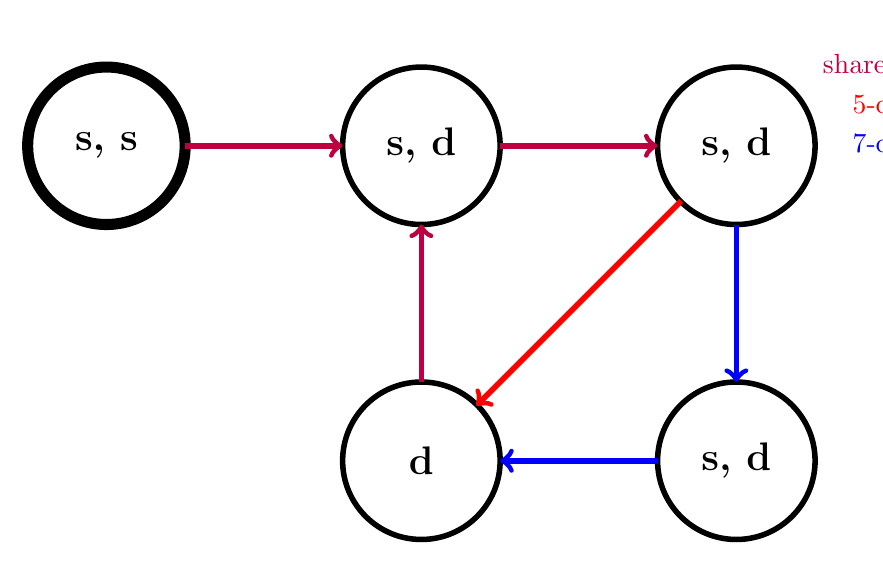
\begin{tikzpicture}
        % Bounding box
        \useasboundingbox (0,0) -- (10.5,6.5);

        % Nodes
        \node[draw=black, line width=4, circle, minimum size=2cm] (ss) at (1,5) {\Large \textbf{s, s}};
        \node[draw=black, line width=2, circle, minimum size=2cm] (sd1) at (5,5) {\Large \textbf{s, d}};
        \node[draw=black, line width=2, circle, minimum size=2cm] (sd2) at (9,5) {\Large \textbf{s, d}};
        \node[draw=black, line width=2, circle, minimum size=2cm] (sd3) at (9,1) {\Large \textbf{s, d}};
        \node[draw=black, line width=2, circle, minimum size=2cm] (d)   at (5,1) {\Large \textbf{d}};

        % Edges
        % Contractive 7-cycle: blue
        \draw[->, line width=2, blue] (9,4) -- (9,2);        % sd2 -> sd3
        \draw[->, line width=2, blue] (8,1) -- (6,1);        % sd3 -> d

        % Expansive 5-cycle: red
        \draw[->, line width=2, red] (8.3,4.3) -- (5.7,1.7); % sd3 -> ss

        % Shared edge (between 5 and 7): purple
        \draw[->, line width=2, purple] (2,5) -- (4,5);       % ss -> sd1
        \draw[->, line width=2, purple] (5,2) -- (5,4);       % d -> sd1
        \draw[->, line width=2, purple] (6,5) -- (8,5);       % sd1 -> sd2

        % Legend
        \node at (11,6)   {\color{purple} shared edge};
        \node at (11,5.5) {\color{red}    5-cycle};
        \node at (11,5)   {\color{blue}   7-cycle};

    \end{tikzpicture}
    \caption{State Transition Diagram for A022921 highlighting cycles: contractive 7-cycle (blue),
    locally expansive 5-cycle (red), shared edges (purple). Lowercase letters reflect single ($s$)
    and double ($d$) parity steps consistent with the main text notation.}
    \label{fig:cycle-highlight-lower}
\end{figure}

The figure highlights the locally expansive 5-cycle (red), the contractive 7-cycle (blue), 
and the shared edges (purple), visually illustrating the grammar constraints of the 
sequence \OEIS{A022921}.

\newpage
\subsection*{Horizontal-Sum Dynamics and Pascal-Type Growth}

The generating rows evolve by a horizontal-sum rule:
\begin{equation}
a_i(n) = a_i(n-1) + a_{i-1}(n), \quad i,n \in \mathbb{N},
\label{eq:horizontal-sum-recurrence}
\end{equation}
so that sequences of single steps exhibit ordinary Pascal--type growth.
Double steps differ in that the terminal entry is duplicated, causing the
final term to appear twice while preserving monotonicity.

Because the grammar forces expansive configurations to appear only within this minimal 5-block,
extremal asymptotic growth is realized by repeated alignment of this block, making it sufficient
to analyze this configuration.  Thus for extremal 5-cycle analysis, the local maximal sequence
(dominating per-pattern growth) is
\[
\{ s, d, s, d, d \}, \{ s, d, s, d, d \},
\]
enumerating occurrences of each admissible local pattern within a 5-cycle.

\subsection*{Admissible Local Patterns}
\label{sec:admissible-patterns}

Within \OEIS{A022921}, only four local configurations occur:
\[
(s, d), \quad (d, d), \quad (s, d, s), \quad (d, d, s).
\]

The associated coefficient counts within a 5-cycle are:
\[
\begin{array}{c|c}
\text{Pattern} & \text{Associated coefficient count} \\
\hline
s,d & 2 \\
d,d & 1 \\
s,d,s & 1 \\
d,d,s & 1
\end{array}
\]

\subsection{Illustrative Extremal Computations}

The generating rows evolve by a horizontal--sum rule (see Equation \ref{eq:horizontal-sum-recurrence})
so that sequences of single steps exhibit ordinary Pascal--type growth.
Double steps differ only in that the terminal entry of the row is duplicated,
causing the final term to appear twice in the generating tuple while preserving
monotonicity of the preceding entries.

These examples are chosen so that each step saturates the inequalities of
Lemma~\ref{lem:controlled-horizontal-growth}, thereby realizing extremal growth. Equalities
shown below should be interpreted as extremal upper-bound realizations rather than
identities valid for all rows.

The following row-by-row computations realize extremal growth for the admissible
local patterns and together determine the sharpest uniform bounds used in
Lemma~\ref{lem:local-growth-bounds}.  Each example illustrates how a local pattern
can saturate its maximal growth factor under the horizontal-sum dynamics.  Let $S$
denote the total sum of entries in the generating row prior to a given local pattern.

\paragraph{Example 1.}
\[
\begin{array}{l}
\textit{Single } a(10) = \underbrace{173}_{\text{sum} := S}:
\underbrace{1,7,25,55,85}_{S}
\end{array}
\]

\[
\begin{array}{l}
\textit{Double } a(11) = \underbrace{476}_{\text{sum} = 3S}:
\underbrace{1,8,33,88}_{S}
\underbrace{173}_{S},
\underbrace{173}_{S}
\end{array}
\]

\[
\begin{array}{l}
\textit{Single } a(12) = \underbrace{961}_{\text{sum} = 9S}:
\underbrace{1,9,42,130}_{2S}
\underbrace{303}_{3S},
\underbrace{476}_{4S}
\end{array}
\]

\[
\begin{array}{l}
\textit{Double } a(13) = \underbrace{2652}_{\text{sum} = 33S}:
\underbrace{1,10,52,182}_{4S},
\underbrace{485}_{7S},
\underbrace{961}_{11S},
\underbrace{961}_{11S}
\end{array}
\]

\[
\begin{array}{l}
\textit{Double } a(14) = \underbrace{8045}_{\text{sum} = 123S}:
\underbrace{1,11,63,245}_{8S},
\underbrace{730}_{15S},
\underbrace{1691}_{26S},
\underbrace{2652}_{37S},
\underbrace{2652}_{37S}
\end{array}
\]

\[
\begin{array}{l}
\textit{Single } a(15) = \underbrace{17637}_{\text{sum} = 329S}:
\underbrace{1,12,75,320}_{16S},
\underbrace{1050}_{31S},
\underbrace{2741}_{57S},
\underbrace{5393}_{94S},
\underbrace{8045}_{131S}
\end{array}
\]

The resulting maximal local ratios are
\[
\begin{array}{c|c}
\text{Pattern} & \text{Max Ratio} \\
\hline
s,d & 3/1 \\
d,d & 123/33 \\
s,d,s & 9/3 \\
d,d,s & 329/123
\end{array}
\]

\paragraph{Example 2.}
\[
\begin{array}{l}
\textit{Single } a(12) = \underbrace{961}_{\text{sum} := S}:
\underbrace{1,9,42,130,303,476}_{S}
\end{array}
\]

\[
\begin{array}{l}
\textit{Double } a(13) = \underbrace{2652}_{\text{sum} = 3S}:
\underbrace{1,10,52,182,485}_{S},
\underbrace{961}_{S},
\underbrace{961}_{S}
\end{array}
\]

\[
\begin{array}{l}
\textit{Double } a(14) = \underbrace{8045}_{\text{sum} = 13S}:
\underbrace{1,11,63,245,730}_{2S},
\underbrace{1691}_{3S},
\underbrace{2652}_{4S},
\underbrace{2652}_{4S}
\end{array}
\]

\[
\begin{array}{l}
\textit{Single } a(15) = \underbrace{17637}_{\text{sum} = 37S}:
\underbrace{1,12,75,320,1050}_{4S},
\underbrace{2741}_{7S},
\underbrace{5393}_{11S},
\underbrace{8045}_{15S}
\end{array}
\]

\[
\begin{array}{l}
\textit{Double } a(16) = \underbrace{51033}_{\text{sum} = 131S}:
\underbrace{1,13,88,408,1458}_{8S},
\underbrace{4199}_{15S},
\underbrace{9592}_{26S},
\underbrace{17637}_{41S},
\underbrace{17637}_{41S}
\end{array}
\]

\[
\begin{array}{l}
\textit{Single } a(17) = \underbrace{108950}_{\text{sum} = 341S}:
\underbrace{1,14,102,510,1968}_{16S},
\underbrace{6167}_{31S},
\underbrace{15759}_{57S},
\underbrace{33396}_{98S},
\underbrace{51033}_{139S}
\end{array}
\]

The corresponding maximal local ratios are
\[
\begin{array}{c|c}
\text{Pattern} & \text{Max Ratio} \\
\hline
s,d & 3/1 \\
d,d & 13/3 \\
s,d,s & 341/131 \\
d,d,s & 37/13
\end{array}
\]

\subsection*{Improved Extremal Alignment}

Because the total multiplicative growth over a cycle is the product of the local
growth factors, the geometric mean over one full cycle is maximized by selecting
the maximal admissible factor at each local pattern occurrence. Consequently,
once a uniform upper bound has been established for each admissible local pattern,
the extremal global growth rate over a complete cycle is obtained by multiplying
these maximal local factors according to their frequencies and taking the
corresponding geometric mean.

\emph{Equivalently, because total growth over any admissible word is multiplicative in
its local factors, the asymptotic per-symbol growth rate is the geometric mean of these
factors;  hence the maximal rate over the entire language generated by the grammar is
achieved by the word that maximizes this mean subject to the grammar constraints.}

Each example yields a valid (not necessarily sharp) upper bound on the maximal growth
factor associated with each admissible local pattern.  Since these bounds arise from
the same uniform recurrence and apply globally to all admissible configurations, the
true maximal growth factor for a given pattern is bounded above by the smallest
recorded bound among all such valid upper bounds.

Because the recurrence is monotone with respect to the placement of delayed doubling,
no other admissible configuration can exceed these extremal realizations.
Accordingly, combining the sharpest bounds obtained across different initiating
rows yields the tightest global envelope on admissible local growth.

\[
\begin{array}{c|c|c}
\text{Pattern} & \text{Max Ratio} & \text{Associated coefficient count} \\
\hline
s,d & 3 & 2 \\
d,d & 123/33 & 1 \\
s,d,s & 341/131 & 1 \\
d,d,s & 329/123 & 1
\end{array}
\]

Consequently, the maximal geometric growth rate of a $5$--cycle satisfies
\begin{equation}
\Bigl(
3^2 \cdot (123/33) \cdot (341/131) \cdot (329/123)
\Bigr)^{1/5} 
\approx 2.976 < 3.
\label{eq:rho-5}
\end{equation}

This bound directly feeds into Theorem~\ref{thm:maximal-growth} and ensures that
the per-symbol growth of any admissible infinite sequence under \OEIS{A186009}
is strictly dominated by $3$, as explained in the main text.

\paragraph{Conclusion.}
Every admissible growth pattern of \OEIS{A186009} is constrained by the grammar
of \OEIS{A022921}. Infinite concatenations of 5-cycles, though forbidden, saturate
local growth constraints and provide a strict upper envelope. Equation~\eqref{eq:rho-5}
confirms that even this extremal envelope has geometric growth rate $< 3$, ensuring
subdominance relative to the denominator $2^{B(i)}$.


\newpage
\section{Horizontal-Sum Table for A186009}
\label{app:horizontal-sum-table}

For reference, a portion of \OEIS{A186009} generated by the horizontal-sum construction is
given below as per an algorithm derived from Winkler \cite{Winkler2017}. This table is included
for illustration of the horizontal-sum mechanism; none of the density or growth bounds in the
main text depend on these specific numeric values.

\begin{table}[htbp]
\centering
\caption{A186009 Horizontal Sum Formulation}
\label{tab:A186009}
\vspace{4pt}
\begin{tabular}{@{}rrrrrrrrrrr@{}}
\toprule
$n$ & $a_1(n)$ & $a_2(n)$ & $a_3(n)$ & $a_4(n)$ & $a_5(n)$ &
$a_6(n)$ & $a_7(n)$ & $a_8(n)$ & $a_9(n)$ & $\sum a_i(n)$ \\
\midrule
1  & 1 &   &   &   &   &   &   &   &   & 1 \\
2  & 1 &   &   &   &   &   &   &   &   & 1 \\
3  & 1 &   &   &   &   &   &   &   &   & 1 \\
4  & 1 & 1 &   &   &   &   &   &   &   & 2 \\
5  & 1 & 2 &   &   &   &   &   &   &   & 3 \\
6  & 1 & 3 & 3 &   &   &   &   &   &   & 7 \\
7  & 1 & 4 & 7 &   &   &   &   &   &   & 12 \\
8  & 1 & 5 & 12 & 12 &   &   &   &   &   & 30 \\
9  & 1 & 6 & 18 & 30 & 30 &   &   &   &   & 85 \\
10 & 1 & 7 & 25 & 55 & 85 &   &   &   &   & 173 \\
11 & 1 & 8 & 33 & 88 & 173 & 173 &   &   &   & 476 \\
12 & 1 & 9 & 42 & 130 & 303 & 476 &   &   &   & 961 \\
13 & 1 & 10 & 52 & 182 & 485 & 961 & 961 &   &   & 2652 \\
14 & 1 & 11 & 63 & 245 & 730 & 1691 & 2652 & 2652 &   & 8045 \\
15 & 1 & 12 & 75 & 320 & 1050 & 2741 & 5393 & 8045 &   & 17637 \\
16 & 1 & 13 & 88 & 408 & 1458 & 4199 & 9592 & 17637 & 17637 & 51033 \\
17 & 1 & 14 & 102 & 510 & 1968 & 6167 & 15759 & 33396 & 51033 & 108950 \\
\bottomrule
\end{tabular}
\end{table}

There is a sequence closely related to \OEIS{A186009} called \OEIS{A100982}.  \OEIS{A186009}
prepends the number 1 to the \OEIS{A100982} sequence.  Along with the listing of initial
terms for \OEIS{A100982} comes an algorithm which explains how to generate the entire sequence
starting with an initial value of 1.  As a result of its close similarity, this method can
also be leveraged to generate all of the terms in \OEIS{A186009}. 

Theorem 2 \cite{Winkler2017} referenced in \OEIS{A100982} asserts that the elements in the
sequence can be derived in a Pascal–triangle–type manner, beginning with an initial condition:
% Starting condition for A100982
\[
a(1) = a_1(1) = 1
\]

The algorithm for $A100982(n)$ states that the $k^{th}$ term of the $n^{th}$ series component
can be computed as follows:
% Recursive algorithm for generating new terms for A100982 based on previously generated terms
\[
a_{k+1}(n) = a_k(n) + a_k(n-1); k \in \setNo, n \in \setN
\]

The algorithm also stipulates that the last term in the sequence is repeated whenever
$A022921(n-2)=2$ (which can be derived from \OEIS{A020914} by taking the first
differences between its terms).  In doing so, this imposes the implicit constraint that this rule
applies only when $n \ge 2$.  Keeping in mind that repeated terms in \OEIS{A022921}
occur only once $n \ge 2$, the recurrence is extended to $n=1$ by treating the duplication
condition as inactive at the boundary, producing an augmented vertical-sum expansion.

In rows without terminal duplication, this recurrence is exactly Pascal’s binomial rule; duplication acts
only at the boundary and therefore preserves the monotone, binomial-type growth of interior entries.
This boundary-only modification is precisely why the extremal growth analysis in
Appendix~\ref{app:local-growth-details} reduces to \emph{local pattern frequencies}
rather than global row shape.

We reformulate this construction such that the first non-zero term in
each row is always at index 1 and thus the formula henceforth (producing the same expansion
components up to a reindexing of coordinates) is modified as follows.

Preserving $a(1) = a_1(1) = a_1(n) = 1 \text{ for all } n\in\setN$, the $i^{th}$ term of the
$n^{th}$ \OEIS{A100982} element is:
% Modified recursive algorithm for generating new terms for A100982 based on previously generated terms
\[
a_{i}(n) = a_i(n-1) + a_{i-1}(n); i,n \in \setN
\]

This reindexing does not change any row sums or terminal-duplication positions; it only relocates coordinates.
Using this formulation the initial term for all values of $n \in \setN$ is always 1 rather than
shifting out for each value of $n$.  The other significant difference is that in this formulation
the values for $a_i(n)$ appear horizontally as opposed to vertically.  The doubling rule for the
terminal entry remains unchanged in substance – namely that it occurs when $A022921(n-2) = 2$ -
which is precisely the single/double grammar governing admissible growth in the preceding appendices,
and hence the local multiplicative structure used in the extremal bounds.

Because \OEIS{A186009} is obtained from \OEIS{A100982} by prepending an initial row, all row indices
shift by one.  Consequently the terminal-duplication condition expressed in the original
formulation as $A022921(n-2)=2$ now becomes $A022921(n-3)=2$ in the present indexing.


\newpage
\section{Enumeration of Admissible Parity Words}
\label{app:parity-enumeration}

\subsection*{Purpose and Scope}

This appendix provides an explicit, constructive procedure for enumerating
admissible parity words of fixed length under the prefix constraints governed by
\OEIS{A020914}.  While none of the density or growth bounds in the main text
depend on these constructions, the algorithm clarifies the combinatorial
structure underlying \OEIS{A186009} and makes explicit the finite grammar
inducing admissible parity words implicit in the horizontal-sum formulation.

\subsection*{Prefix-Sum Formulation}

Let a parity word of length $m \ge 1$ be a tuple
\[
(d_0,d_1,\dots,d_{m-1}), \qquad d_i \in \mathbb{N},
\]
where $d_i$ records the number of divisions by $2$ following the $i$th odd step.
Define the prefix sums
\[
H(i) = \sum_{j=0}^{i} d_j .
\]

Admissible parity words of length $m$ are exactly those satisfying

\[
H(i) < A020914(i+1) \quad (0 \le i < m-1), 
\qquad
H(m-1) = A020914(m).
\]

The strict inequalities for $i<m-1$ suppress shorter stopping-time words,
while equality in the final column ensures the total division count matches
the minimal exponent associated with length $m$.

Thus admissible parity words are determined by a bounded prefix-sum search
with backtracking.


\subsection*{Constructive Enumeration Procedure}

Fix a word length $m \ge 1$ and define $m$ columns numbered $i=0,\dots,m-1$.
Below each $i$ calculate the parity word grammar bounds $A(i+1)=A020914(i+1)$.

Then, under each column, place the exponent entries $d_i$ of the parity word.
The left-to-right horizontal sum $H(i)$ is the sum of entries up to column $i$,
where $H(i)$ must satisfy the admissibility bounds described above.


\subsection*{Iterative Search}
Generation of the set of all parity words of length $m$ proceeds by iterating
through the following steps until all admissible words have been found.

Set $i=0$ and $H(-1)=0$ as the initial boundary condition.  Begin at step \ref{step1}.

\begin{enumerate}

\item Set successive row entries $d_i=1$ up to column $m-2$:
\label{step1}
\begin{enumerate}
  \item If $i<m-1$, set $d_i=1$.
  Increment $i$ and repeat Step~\ref{step1}.
  \item Otherwise, proceed to Step~\ref{step2}.
\end{enumerate}

\item Calculate the final entry $d_{m-1}$ so that the horizontal sum matches $A(m)$:
\label{step2}
\[
d_{m-1} = A(m) - H(m-2),
\]
record the resulting parity word $(d_0,\dots,d_{m-1})$. Continue to step \ref{step3}.

\item Increment the $(i-1)^{th}$ column if this is admissible by the grammar:
\label{step3}
\begin{enumerate}
  \item If $H(i-1) < A(i) - 1$, copy the previous row entries up to $i-2$.

  Increment $d_{i-1}$ by 1, and return to Step~\ref{step1}.
  \item Otherwise, proceed to Step~\ref{step4}.
\end{enumerate}

\item Check the termination condition for the parity word search:
\label{step4}

\begin{enumerate}
  \item If $i$ is greater than 1, decrement $i$ by one and return to Step~\ref{step3}.
  \item Otherwise, all admissible parity words of length $m$ have been generated.  Stop.
\end{enumerate}

\end{enumerate}


\subsection*{Example: Parity Words of Length $m=5$}

For $m=5$, the bounds are
\[
A020914(1{:}5) = (2,4,5,7,8).
\]
All admissible parity words must satisfy
\[
H(0)<2,\; H(1)<4,\; H(2)<5,\; H(3)<7,\; H(4)=8.
\]

The search procedure yields the seven admissible words shown in
Table~\ref{tab:m5-words}.

\begin{table}[h]
\centering
\caption{Admissible parity words of length $m=5$.}
\label{tab:m5-words}
\vspace{4pt}
\begin{tabular}{c|ccccc}
$i$ & $0$ & $1$ & $2$ & $3$ & $4$ \\
$A(i+1)$ & $2$ & $4$ & $5$ & $7$ & $8$ \\ \hline
\textbf{Word} & $d_0$ & $d_1$ & $d_2$ & $d_3$ & $d_4$ \\ \hline
1 & 1 & 1 & 1 & 1 & 4 \\
2 & 1 & 1 & 1 & 2 & 3 \\
3 & 1 & 1 & 1 & 3 & 2 \\
4 & 1 & 1 & 2 & 1 & 3 \\
5 & 1 & 1 & 2 & 2 & 2 \\
6 & 1 & 2 & 1 & 1 & 3 \\
7 & 1 & 2 & 1 & 2 & 2 \\
\end{tabular}
\end{table}

Thus $A186009(m+1)=7$ counts admissible parity words of length $m=5$.  
The final word $(1,2,1,2,2)$ is extremal in the sense that its prefix sums
approach the bounds $A020914(i+1)$ as closely as possible for $i<m-1$
while remaining admissible, and achieve equality at $i=m-1$.


\newpage
\section{A Binomial Lower Comparison for A186009}
\label{app:A047749-lower-bound}

The sequence \OEIS{A047749} admits a horizontal-sum construction analogous to that
of \OEIS{A186009}, but with a stricter terminal rule: its doubling mechanism is
governed by \OEIS{A000034}$(n-2)$ rather than \OEIS{A022921}. As a result,
\OEIS{A047749} forbids \emph{consecutive} doublings, while such events occur
periodically in \OEIS{A186009}. This structural restriction yields a natural
comparison sequence.

\subsection*{Pointwise comparison}

Because \OEIS{A047749} evolves under the same Pascal-type recursion but with a
subset of the admissible doubling events, its row sums form a pointwise lower
bound (up to index shift):
\[
A047749(n) \le A186009(n+1), \qquad n \ge 0.
\]
The two sequences agree initially, but diverge once the first consecutive
doubling occurs in \OEIS{A186009}; thereafter the inequality is strict.

\subsection*{Closed form for \OEIS{A047749}}

Unlike \OEIS{A186009}, the restricted doubling grammar of \OEIS{A047749}
permits an exact description. Its terms split naturally into even and odd
indices:

\paragraph{Even indices ($n=2m$).}
\[
a(n) = \frac{1}{2m+1}\binom{3m}{m}.
\]

\paragraph{Odd indices ($n=2m+1$).}
\[
a(n) = \frac{1}{2m+1}\binom{3m+1}{m+1}.
\]

Equivalently, using Gamma functions,
\[
a(2m)=\frac{\Gamma(3m+1)}{\Gamma(2m+2)\Gamma(m+1)}, \qquad
a(2m+1)=\frac{\Gamma(3m+2)}{\Gamma(2m+2)\Gamma(m+2)}.
\]

\subsection*{Asymptotic growth}

Let $\psi(x)=\Gamma'(x)/\Gamma(x)$ be the digamma function. Differentiating the
logarithm of the Gamma representations gives

\[
\frac{d}{dm}\ln a(2m)
  = 3\psi(3m+1)-2\psi(2m+2)-\psi(m+1),
\]
\[
\frac{d}{dm}\ln a(2m+1)
  = 3\psi(3m+2)-2\psi(2m+2)-\psi(m+2).
\]

Using $\psi(x)=\ln x + O(1/x)$ as $x\to\infty$,
both expressions have the same limit:
\[
\lim_{m\to\infty} \frac{d}{dm}\ln a(n)
= \ln\!\left(\frac{3^3}{2^2}\right)
= \ln\!\left(\frac{27}{4}\right).
\]

Thus
\[
\lim_{n\to\infty}\frac{a(n+2)}{a(n)}=\frac{27}{4},
\qquad
a(n) \sim C\left(\sqrt{\frac{27}{4}}\right)^n.
\]

\subsection*{Implication for \OEIS{A186009}}

Since \OEIS{A047749} is generated by a subset of the admissible doubling events
for \OEIS{A186009}, it provides a constructive comparison sequence with
explicit exponential growth rate
\[
\sqrt{\frac{27}{4}} = \frac{3\sqrt{3}}{2} \approx 2.598.
\]
Hence \OEIS{A186009} admits an explicit exponentially growing comparison sequence,
and grows strictly faster once consecutive doubling regimes become active.


\clearpage
\bibliographystyle{unsrtnat}
\bibliography{src/latex/references}

\end{document}  
